\documentclass{article}

\usepackage{Sweave}
\usepackage[utf8]{inputenc}
\usepackage{color}
\usepackage{amssymb}
\usepackage{amsmath}
\usepackage{color}
\RequirePackage{/Library/Frameworks/R.framework/Versions/3.2/Resources/library/BiocStyle/resources/tex/Bioconductor}

\AtBeginDocument{\bibliographystyle{/Library/Frameworks/R.framework/Versions/3.2/Resources/library/BiocStyle/resources/tex/unsrturl}}


\title{`Fragmentation duplicates': Sweave}
\author{Andy Lynch and Mike Smith}
\begin{document}
\Sconcordance{concordance:duplicatessweave.tex:duplicatessweave.Rnw:%
1 7 1 1 2 1 0 1 3 17 1}
\Sconcordance{concordance:duplicatessweave.tex:./ChildRNW/Child1-Introduction.Rnw:ofs 28:%
1 11 1 1 2 11 0 1 2 25 1 1 2 1 0 3 1 3 0 1 2}
\Sconcordance{concordance:duplicatessweave.tex:duplicatessweave.Rnw:ofs 87:%
32 2 1}
\Sconcordance{concordance:duplicatessweave.tex:./ChildRNW/Child2-UsePackage.Rnw:ofs 90:%
1 9 1 1 2 4 0 1 2 6 1 1 2 4 0 1 2 1 1}
\Sconcordance{concordance:duplicatessweave.tex:duplicatessweave.Rnw:ofs 119:%
36 2 1}
\Sconcordance{concordance:duplicatessweave.tex:./ChildRNW/Child3-Methods.Rnw:ofs 122:%
1 318 1}
\Sconcordance{concordance:duplicatessweave.tex:duplicatessweave.Rnw:ofs 441:%
40 2 1}
\Sconcordance{concordance:duplicatessweave.tex:./ChildRNW/Child4-Simulations.Rnw:ofs 444:%
1 23 1 1 2 1 0 3 1 10 0 1 2 15 1 1 2 1 0 1 1 1 2 1 1 1 3 1 1 6 0 1 1 7 0 1 2 2 1 %
1 2 1 0 3 1 3 0 1 2 4 1 1 2 1 0 2 1 1 2 1 1 8 0 1 2 6 1 1 2 1 0 5 1 1 2 1 1 11 0 %
2 2 1 0 3 1 3 0 1 2 6 1 1 2 1 0 1 1 1 3 7 0 1 4 4 1 1 2 1 0 9 1 1 2 1 1 15 0 1 2 %
2 1 1 2 1 0 3 1 3 0 1 2 3 1}
\Sconcordance{concordance:duplicatessweave.tex:duplicatessweave.Rnw:ofs 652:%
44 3 1}
\Sconcordance{concordance:duplicatessweave.tex:./ChildRNW/Child5-SNPchoice.Rnw:ofs 656:%
1 13 1 1 2 4 0 1 2 6 1 1 2 1 0 1 2 1 0 3 1 3 0 1 2 7 1 1 2 1 0 1 1 1 3 5 0 1 2 3 %
1 1 2 1 0 1 6 8 0 1 2 3 1 1 2 1 0 3 1 1 5 3 0 1 6 5 0 2 1 3 0 1 2 4 1 1 2 11 0 1 %
2 2 1}
\Sconcordance{concordance:duplicatessweave.tex:duplicatessweave.Rnw:ofs 768:%
49 4 1}
\Sconcordance{concordance:duplicatessweave.tex:./ChildRNW/Child6-Samples.Rnw:ofs 773:%
1 20 1 1 2 1 0 4 1 3 0 1 2 5 1 1 2 1 0 1 1 3 0 1 2 2 1 1 2 1 0 4 1 35 0 1 2 2 1 %
1 2 8 0 2 1 3 0 1 2 4 1 1 2 8 0 5 1 5 0 1 2 1 0 1 1 3 0 1 2 8 1 1 2 1 0 1 1 1 8 %
9 0 1 2 2 1 1 2 1 0 2 1 3 0 1 2 5 1 1 2 1 0 1 1 1 5 4 0 4 1 21 0 1 2 1 1}
\Sconcordance{concordance:duplicatessweave.tex:duplicatessweave.Rnw:ofs 979:%
55 2 1}
\Sconcordance{concordance:duplicatessweave.tex:./ChildRNW/Child7-SNPnumbers.Rnw:ofs 982:%
1 7 1 1 2 1 0 1 1 1 2 3 1 3 0 1 2 6 1 1 2 4 0 1 2 2 1 1 2 4 0 1 2 2 1 1 2 4 0 1 %
2 4 1 1 2 8 0 1 2 2 1 1 2 23 0 1 1 15 0 1 2 4 1 1 3 9 0 1 2 1 1 1 2 26 0 1 2 5 1 %
1 2 7 0 1 2 2 1 1 2 6 0 1 1 6 0 1 2 1 1 1 2 6 0 1 1 6 0 1 2 1 1 1 2 6 0 1 1 6 0 %
1 2 1 1 1 2 7 0 1 2}
\Sconcordance{concordance:duplicatessweave.tex:duplicatessweave.Rnw:ofs 1203:%
59 3 1}
\Sconcordance{concordance:duplicatessweave.tex:./ChildRNW/Child8-DuplicateRates.Rnw:ofs 1207:%
1 6 1 1 2 1 0 3 1 28 0 1 2 4 1 1 3 2 0 1 2 4 0 1 2 3 1 1 2 1 0 1 2 1 5 4 0 2 1 1 %
2 2 1 3 0 1 2 8 1 1 2 12 0 1 2 2 1 1 2 12 0}
\Sconcordance{concordance:duplicatessweave.tex:duplicatessweave.Rnw:ofs 1318:%
64 2 1}
\Sconcordance{concordance:duplicatessweave.tex:./ChildRNW/Child9-Consistency.Rnw:ofs 1321:%
1 5 1 1 2 1 0 1 1 1 2 4 0 1 3 2 1 1 3 1 0 1 1 1 2 4 0 1 3 3 1 1 3 2 0 1 1 3 0 1 %
2 7 1 1 2 1 0 1 1 3 0 1 2 3 1 1 2 1 0 1 1 3 0 1 2 2 1 1 3 2 0 1 1 3 0 1 2 2 1}
\Sconcordance{concordance:duplicatessweave.tex:duplicatessweave.Rnw:ofs 1394:%
68 2 1}
\Sconcordance{concordance:duplicatessweave.tex:./ChildRNW/Child11-SingleEnd.Rnw:ofs 1397:%
1 5 1 1 2 1 0 1 1 3 0 2 2 1 0 2 1 12 0 1 2 4 1 1 2 1 0 4 1 3 0 1 2 1 1 1 2 1 0 1 %
2 2 1 1 2 1 1 3 0 1 2 1 1}
\Sconcordance{concordance:duplicatessweave.tex:duplicatessweave.Rnw:ofs 1454:%
72 4 1}
\Sconcordance{concordance:duplicatessweave.tex:./ChildRNW/Child12-Tumour.Rnw:ofs 1459:%
1 16 1 1 2 1 0 1 1 16 0 1 2 7 0 1 2 4 1 1 2 1 0 1 1 3 0 1 2 5 1 1 3 1 0 3 1 3 0 %
1 2 2 1 1 4 3 0 4 1 3 0 1 2 4 1 1 2 4 0 1 2 2 1 1 2 9 0 1 2 25 1}
\Sconcordance{concordance:duplicatessweave.tex:duplicatessweave.Rnw:ofs 1591:%
78 3 1}
\Sconcordance{concordance:duplicatessweave.tex:./ChildRNW/Child13-Complexity.Rnw:ofs 1595:%
1 12 1 1 2 1 0 1 1 7 0 1 2 6 1 1 2 1 0 1 4 6 0 1 2 2 1 1 2 1 0 1 6 5 0 1 1 7 0 1 %
2 7 1 1 2 1 0 1 6 5 0 1 1 7 0 1 2 4 1 1 2 8 0 1 2}
\Sconcordance{concordance:duplicatessweave.tex:duplicatessweave.Rnw:ofs 1692:%
83 3 1}
\Sconcordance{concordance:duplicatessweave.tex:./ChildRNW/Child10-ByLane.Rnw:ofs 1696:%
1 3 1 1 2 1 0 1 1 5 0 1 1 6 0 1 2 2 1 1 6 5 0 1 1 1 2 3 0 1 2 2 1 1 2 1 0 1 1 3 %
0 1 2 2 1 1 2 1 0 1 4 6 0 1 2 3 1 1 2 1 0 1 6 5 0 1 1 5 0 1 1 6 0 1 2 2 1 1 2 1 %
0 1 6 5 0 1 1 5 0 1 1 6 0 1 2 2 1 1 2 1 0 3 1 1 3 2 0 1 5 4 0 1 3 2 0 1 3 3 1 3 %
0 1 2 2 1}
\Sconcordance{concordance:duplicatessweave.tex:duplicatessweave.Rnw:ofs 1828:%
88 3 1}
\Sconcordance{concordance:duplicatessweave.tex:./ChildRNW/Child14-Mitochondria.Rnw:ofs 1832:%
1 7 1 1 2 1 0 10 1 1 2 9 1 1 2 9 1 3 0 1 2 8 1 1 2 1 0 1 1 3 0 1 2 2 1 1 2 7 0 1 %
1 7 0 1 2 2 1 1 2 1 0 1 2 4 0 1 3 2 1 1 2 1 0 5 1 1 2 3 1 1 3 2 1 1 3 2 0 1 5 4 %
0 1 1 3 0 1 2 2 1}
\Sconcordance{concordance:duplicatessweave.tex:duplicatessweave.Rnw:ofs 1951:%
93 5 1 1 2 18 0 1 2 1 1}


\maketitle
\tableofcontents





\clearpage{}

\section{Introduction: The LynchSmithEldridgeTavareFragDup Package}
% !Rnw root = duplicatessweave.Rnw

\subsection{This Sweave}

After offering guidance on using the package, this Sweave generates the tables and data-driven figures displayed in the paper `A method for the empirical correction of estimated PCR duplication rates, with applications' by Lynch, Smith, Eldridge and Taver\'{e} on behalf of the OCCAMS Consortium. It also provides greater information on some points of detail. It is dependent on the \Bioconductor{} \Biocpkg{BiocStyle} package.

This Sweave is part of the \R{} package \Rpackage{FragmentationDuplicates} that provides functionality for the methods described in that paper. 

\subsection{The Data}

The contents of the extdata folder in the package are:

\begin{Schunk}
\begin{Sinput}
> list.files(system.file("extdata", package="FragmentationDuplicates"))
\end{Sinput}
\begin{Soutput}
 [1] "HetSNPDups.txt"            "HetSNPDupsByLane.txt"      "HetSNPDupsHighGC.txt"     
 [4] "HetSNPDupsLowGC.txt"       "HetSNPTableSingleEnd.tsv"  "HetSNPTableTumourAABB.tsv"
 [7] "HetSNPTableTumourAB.tsv"   "HSTtest.tsv"               "ISDs"                     
[10] "masks"                     "Picard"                    "SNPstoextract.txt"        
[13] "Tumour"                    "WeaverSuppTable1.txt"     
\end{Soutput}
\end{Schunk}

\file{WeaverSuppTable1.txt} reproduces data from the first Supplementary Table of Weaver et al. (2014) \emph{Nature Genetics} \textbf{46}, 837-843, and describes the samples used to illustrate this manuscript.

The files \file{HetSNPDups.txt}, \file{HetSNPDupsByLane.txt}, \file{HetSNPDupsHighGC.txt}, \file{HetSNPDupsLowGC.txt}, \file{HetSNPTableSingleEnd.tsv}, \file{HetSNPTableTumourAABB.tsv}, \file{HetSNPTableTumourAB.tsv}, \file{HSTtest.tsv} give tables of allele patterns from duplicate-fragment-sets for various BAM file and SNP combinations (the last file in that list being an artificial case) and are used through this vignette.

\file{SNPstoextract.txt} gives details of the SNPs described in Section~\ref{sec:SNPs}.

The contents of \file{masks} and \file{Picard} detail the numbers of reads and duplicates within defined regions of the genome as discussed in Section~\ref{sec:SampInfo}, while the contents of \file{Tumour} are used in Section~\ref{sec:Tumour}. \file{ISDs} contains details of the insert size distributions for the samples we are considering in this study.


\subsection{The Functions}

The library defines several functions including the following key ones:

\begin{itemize}
  \item \Rfunction{processBAMfordups}: a function to process a BAM file (or BAM files) and produce a table detailing the allele patterns of all observed duplicate fragment-sets. More details are given in the next section.
  \item \Rfunction{processduptable}: a function that processes the output of \Rfunction{processBAMfordups} and returns estimates of the duplicate rates broken down into PCR and fragmentation duplicates. More details are given in the next section.
    \item \Rfunction{genPL}: Generate the lists of all partitions of $M$ objects.
    \item \Rfunction{genCoefs}: Generates the coefficients associated with partitions of objects.
\end{itemize}


\subsection{Preparations}

There are a few steps that we must take before we begin.

\begin{Schunk}
\begin{Sinput}
> library("xtable")
> library("Rsamtools")
> library("BSgenome.Hsapiens.UCSC.hg19")
> EDpath <- system.file("extdata", package="FragmentationDuplicates")
\end{Sinput}
\end{Schunk}

\clearpage{}

\section{General use of the package}
% !Rnw root = duplicatessweave.Rnw

There are two primary functions provided to the user in this package. \Rfunction{processBAMfordups} takes an input BAM file and returns a table of allele patterns observed in sets of duplicate reads, while \Rfunction{processduptable} takes such a table and makes inference about the duplication rates.

\subsection{\Rfunction{processBAMfordups}}

This function takes as its arguments a list of BAM files to process, the path in which to find them, and a list of locations at which to look for heterozygous SNPs. The BAM files must be indexed and have had duplicate reads marked (by e.g. Picard). Other parameters specifying the format of the list of locations, and the criteria by which to accept a locus for use in the analysis can also be set.

The usage is as follows:

\begin{Schunk}
\begin{Sinput}
> duptable<-processBAMfordups(bamfilelist,path,snplist)
\end{Sinput}
\end{Schunk}

The output is a table, the first three columns of which are set as 1) The number of loci deemed to be heterozygous SNPs and therefore of use, 2) the number of well-mapped reads covering those loci and, 3) the number of duplicates at those loci in which allele patterns could be examined.  Subsequent columns give counts for observed allele patterns (the pattern indicated by the column name), while the final column indicates the count of reads that had an inconsistent allele call at the relevant locus.

\subsection{\Rfunction{processduptable}}

The second key function takes the output of processBAMfordups and processes it to estimate the fraction of duplicates attributable to fragmentation.

\begin{Schunk}
\begin{Sinput}
> processduptable(duptable,partitionList,coefficientList)
\end{Sinput}
\end{Schunk}

This outputs a table with a) and estimate of the duplicate rate (but note there will probably be an estimate of this available to the user that is based on more data than are made use of here), b) the proportion of duplicates that are attributable to coincidental fragmentation, c) the resulting estimated PCR duplicate rate, and d) the resulting estimated fragmentation duplicate rate.
\clearpage{}

\section{Methods}
% !Rnw root = duplicatessweave.Rnw



The manuscript that this package accompanies is concerned with separating the observed duplicate rate into a proportion due to PCR duplication of the same original molecule $P_D$, and the proportion due to identical fragmentation of two distinct molecules $F_D = 1-P_D$. To do this we make use of sites of heterogenous SNPs where we can (at least some of the time) distinguish the two scenarios.

\subsection{Case 1: A pair of duplicate fragments}

Recall that if we have only observe duplicate fragments in pairs then, if we observe counts of $N_{AA}$ fragment pairs reporting the same nucleotide, and $N_{AB}$ reporting different nucleotides, the estimate of $P_D$ is
\begin{equation} \label{eq:M2}
P_D = 1- 2 \times N_{AB}/N.
\end{equation} 

\subsection{Case 2: More than two duplicate fragments}
\label{subsec:Case2}

Recall that in this case we estimate $P_D$ by maximizing the total log-likelihood 
\begin{equation}
l(P_D) = \sum_{M} l_M(P_D) .
\end{equation}
\noindent where
\begin{equation}
l_M(P_D) = \sum_{k=1}^{Q_M} N(AP_k) \log\Pr(AP_k \mid P_D),
\end{equation}
\noindent and
\begin{equation}
\Pr(AP_k \mid P_D) = \sum_{i}\Pr(AP_k \mid \text{PART}_i)\Pr(\text{PART}_i \mid P_D).
\end{equation}

In these equations, $M$ is the size of our set of duplicate fragments, $\text{PART}_i$ is the $i^{th}$ potential partition of the duplicate fragments into the original molecules, $AP_k$ is the $k^{th}$ observable allele pattern, and $N(AP_k)$ is the number of times that the allele pattern has been observed.

A worked example for M=4 is given in the main manuscript. An example for M=5 appears in Figure \ref{M5example}.

\begin{figure*}[hp!]
\begin{center}
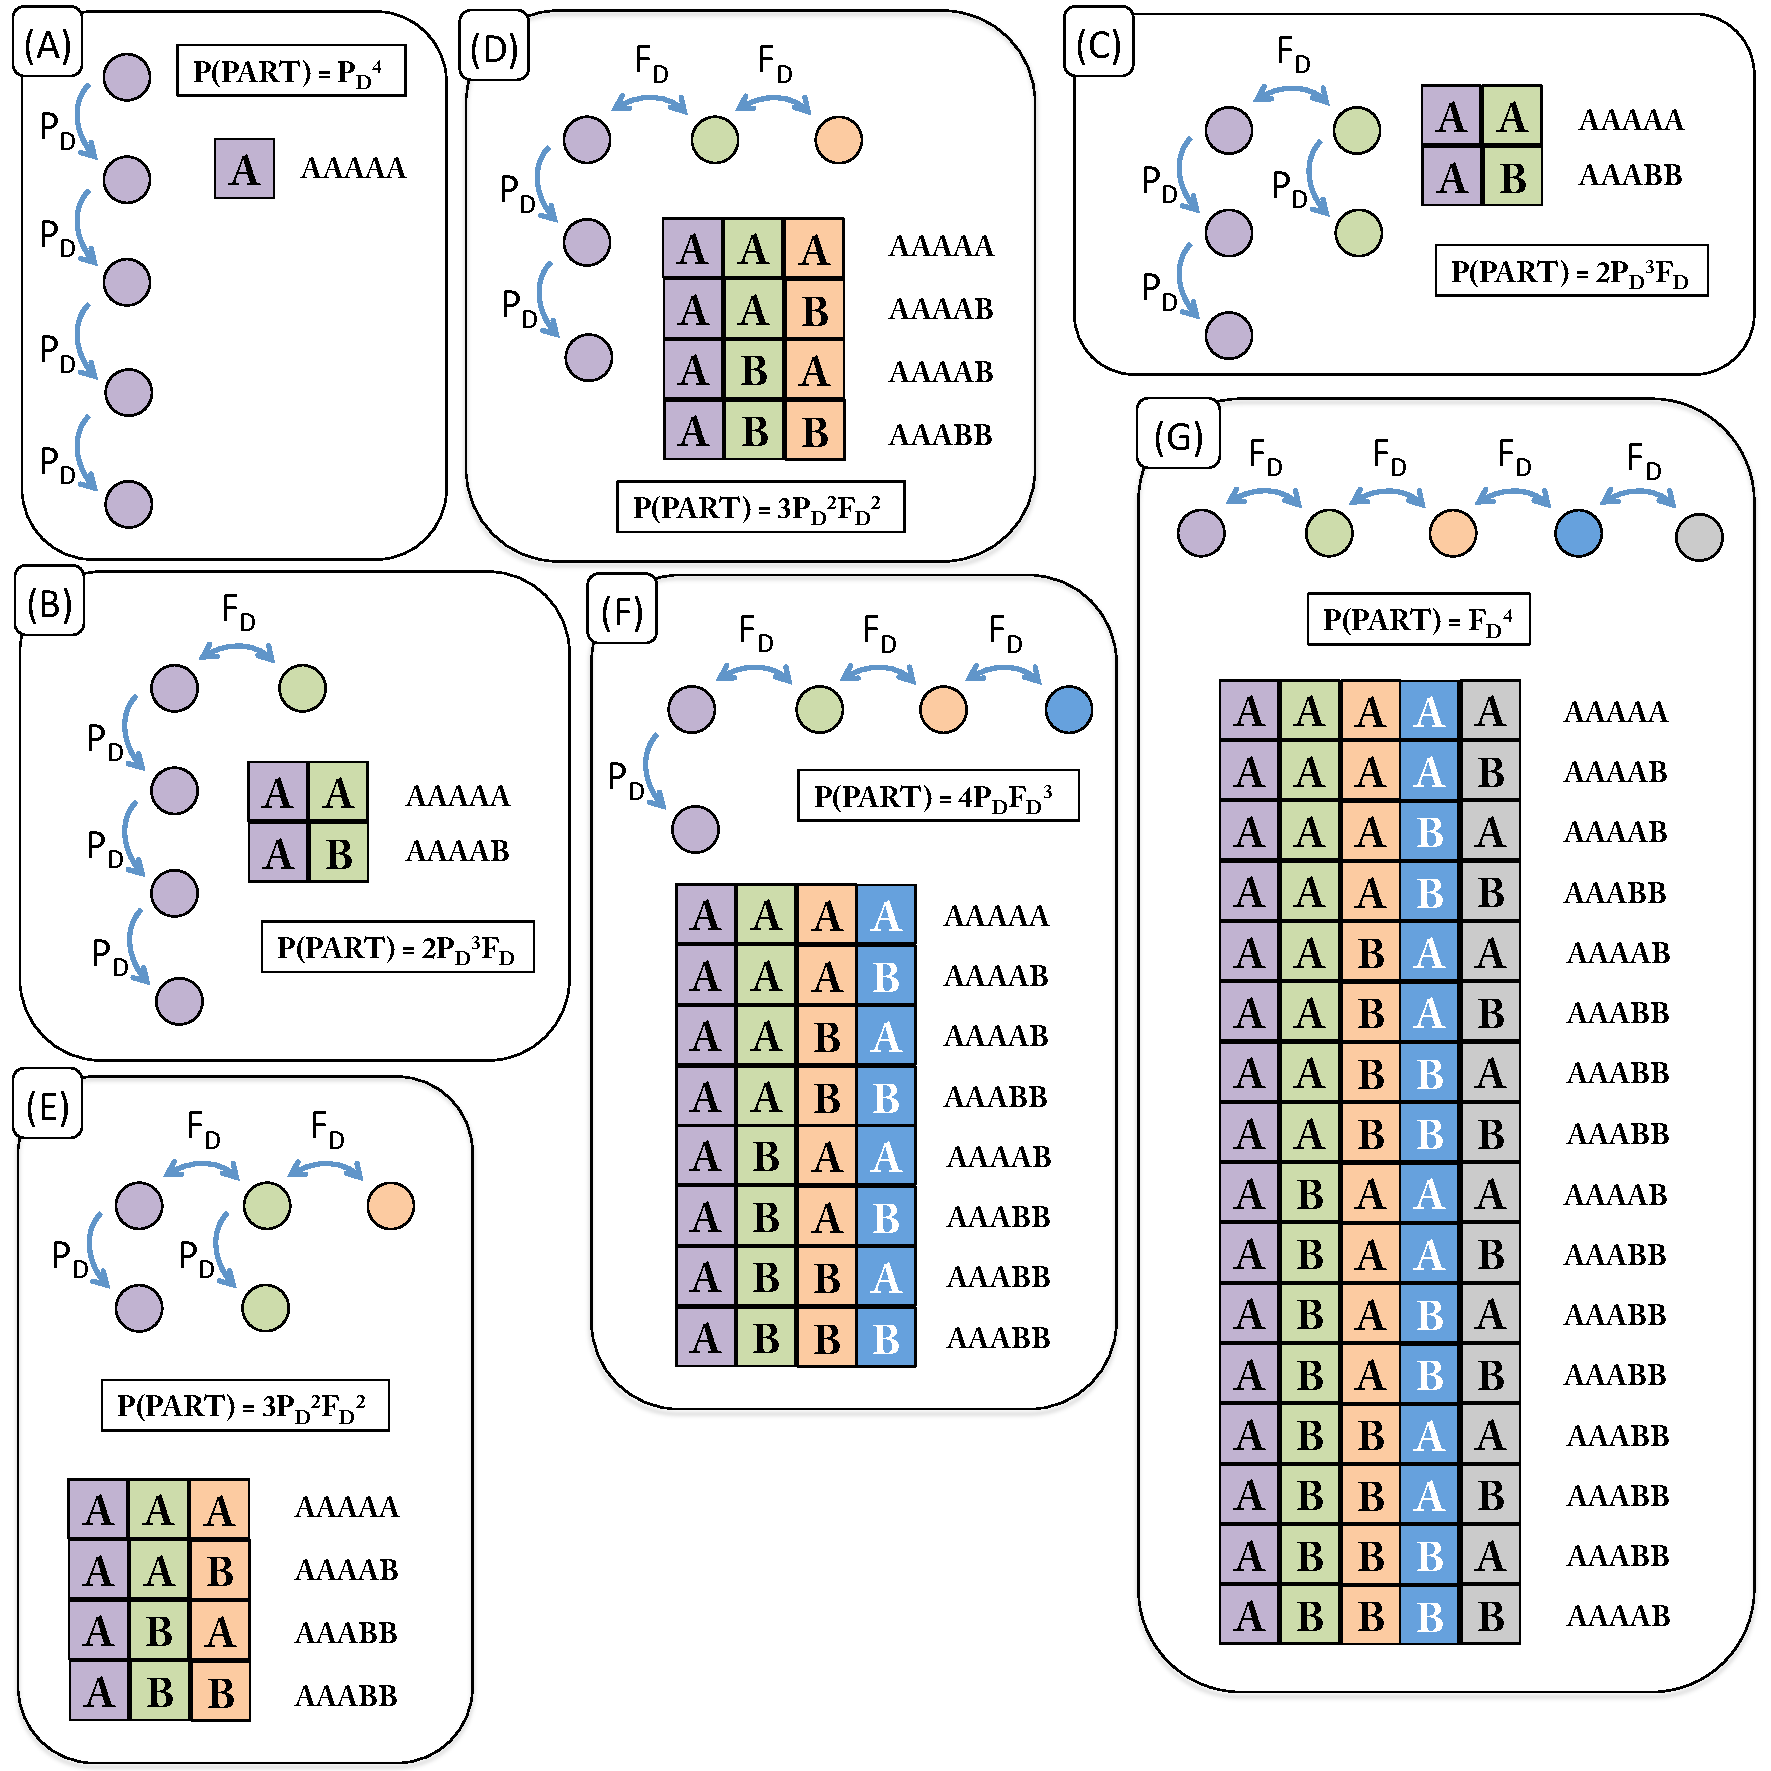
\includegraphics[width=\textwidth]{M5figureexample.pdf}
\end{center}
\caption{Worked example calculation of $\Pr(AP_k \mid P_D)$ for $M = 5$. There are seven identifiably distinct partitions of fragments into molecules. In panel A we have four PCR duplicates of a single fragment. In panel B there are two distinct duplicate fragments, one of which has three PCR duplicates, while panel C has two distinct duplicate fragments one of which has one PCR duplicate and one of which has two PCR duplicates. In panel D, there are three distinct duplicate fragments, one of which has two PCR duplicates and in panel E there are again three distinct fragments, two of which have a PCR duplicate. Panel F depicts the case where there are four distinct molecules, one of which has a PCR duplicate, and in panel G there are five distinct molecules with no PCR duplicates. The probabilities of the seven possible partitions $\Pr(\text{PART}_i \mid P_D)$ are shown, and for each partition the proportions in which the three possible observable allele patterns (AAAAA, AAAAB, AAABB) will arise are illustrated, allowing calculation of $\Pr(AP_k \mid P_D)$  For example $\Pr(\text{AAABB} \mid P_D) = P_D^3F_D + \frac{3}{4}P_D^2F_D^2
+ \frac{3}{2}P_D^2F_D^2 + 2P_DF_D^3 + \frac{10}{16}F_D^4$
}
\label{M5example}
\end{figure*}

The probabilities $\Pr(\text{PART}_i \mid P_D)$ are all of the form $aP_D^bF_D^c$ where $a$, $b$ and $c$ are to be determined. $b$ is clearly the number of PCR duplicates in the partition, and $c = M - b - 1$. 

The calculation of $a$ is not as obvious. Given a partition of the $M$ fragments into $N$ molecules that provide $f_1$,$f_2$,...,$f_N$ fragments in turn ($f_i > 0 \forall i, \sum_i f_i = M$), we denote as $\nu_j$ the number of molecules contributing $j$ fragments $1 \leq j \leq M$. The value of $a$ is then calculated as $a = N!/\prod_j \left( \nu_j! \right) = \left( \sum_j  \nu_j \right)!/\prod_j \left( \nu_j! \right)$. 

To give a concrete example: When there are four fragments ($M = 4$) partitioned amongst three molecules ($N=3$) such that $f_1 = 2$, $f_2 = 1$, and $f_3 = 1$, then  $\nu_1 = 2$  and $\nu_2 = 1$ ($\nu_j =0 \forall j>2$). The value of $a$ is then $3!/(2!1!)=3$.

When M=2 the partition probabilities are not controversial, being $P_D$ if a PCR duplicate is present and $F_D$ if two molecules are present. These probabilities sum to 1 as required. In each case we can consider the addition of a third fragment (a PCR duplicate with probability $P_D$ or a fragmentation duplicate with probability $F_D$). If the new fragment is a PCR duplicate, then it may be a duplicate of any of the existing molecules with equal probability and so the probabilities are shared accordingly. The recursive calculation of these values up to $M=4$ is illustrated in Figure \ref{probderive}.




\begin{figure*}[t]
\begin{center}
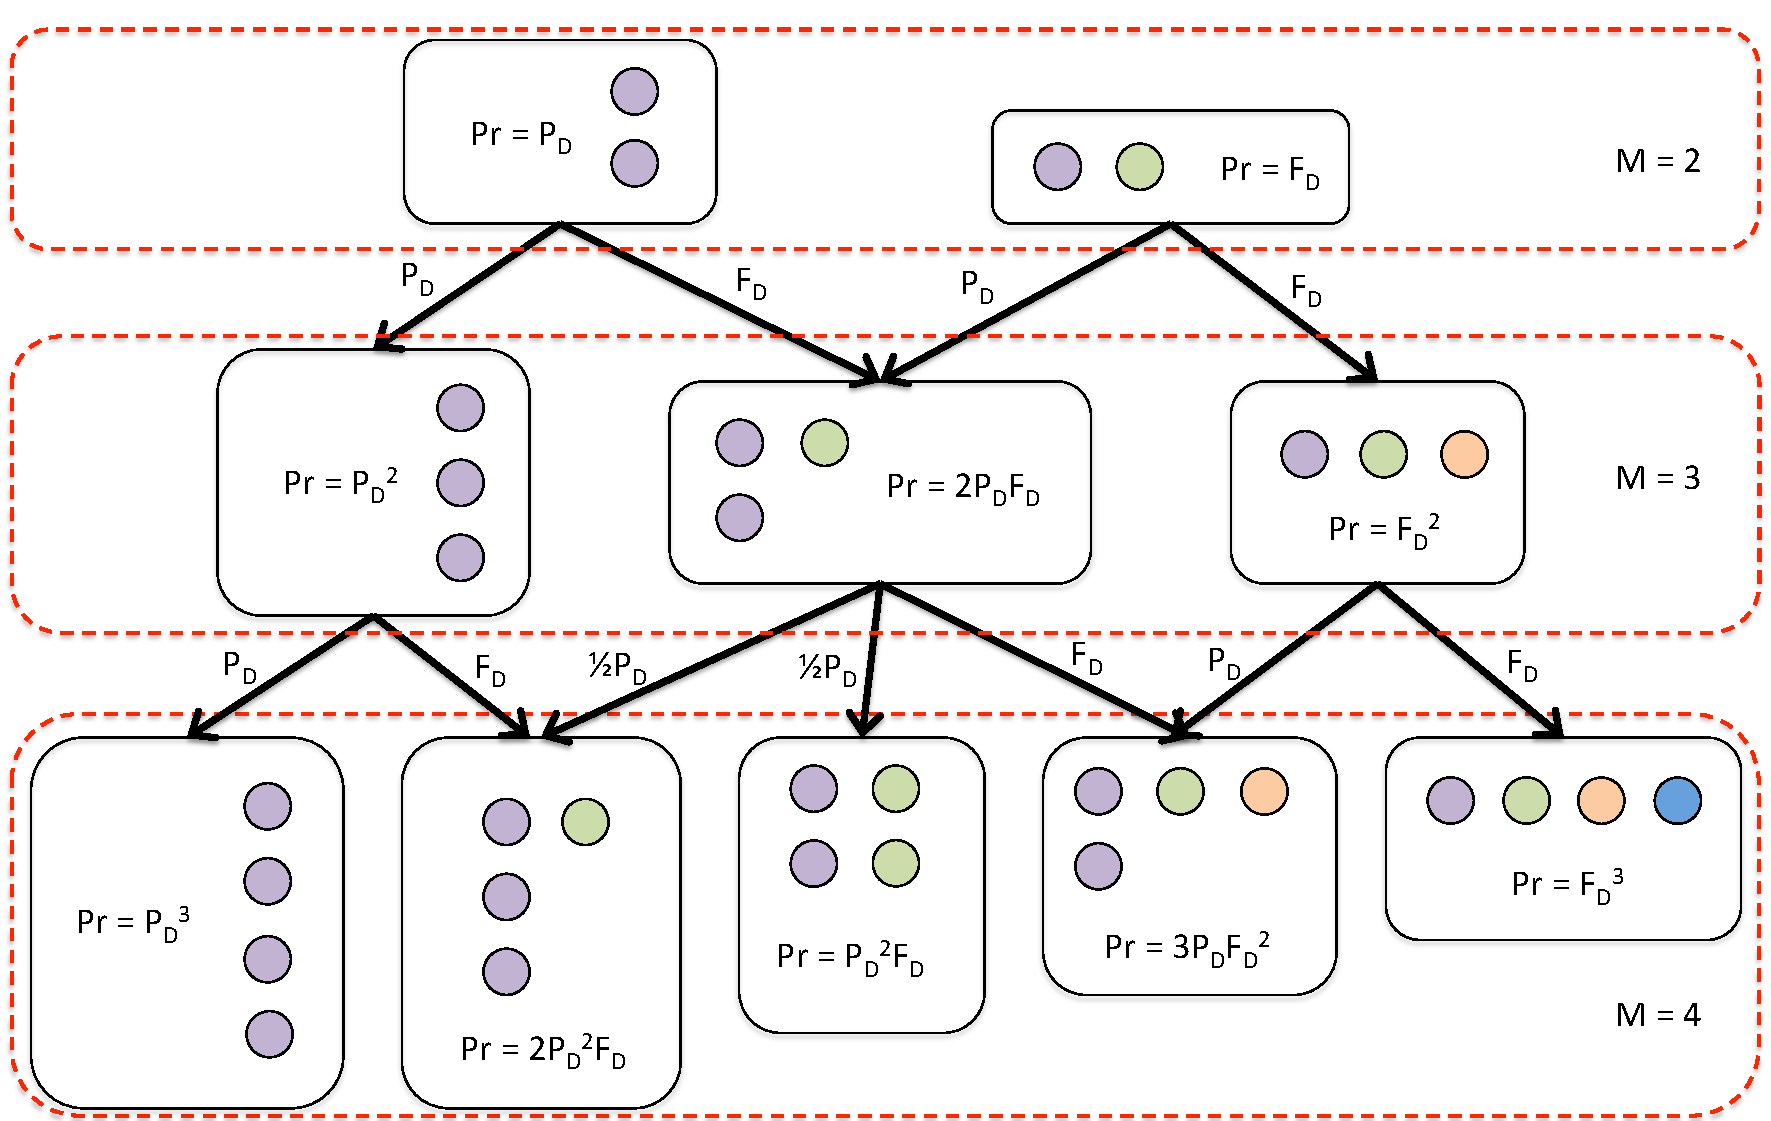
\includegraphics[width=\textwidth]{probderive.pdf}
\end{center}
\caption{Recursive calculation of partition probabilities}
\label{probderive}
\end{figure*}


\subsection{Proof that $a = \left( \sum_j  \nu_j \right)!/\prod_j \left( \nu_j! \right)$}

Given the recursive nature in which we have discussed the calculation of $a$, it is no surprise that the proof is by induction

\subsubsection{The base case (M = 2)}

If M = 2, we either have the left-hand case in Figure~\ref{probderive} where two fragments from the same starting molecule are observed (and so $\nu_2=1, \nu_j =0 \forall j s.t. j \neq 2$), or we have the right hand case where one fragment is observed from each of two original molecules (and so $\nu_1=2, \nu_j =0 \forall j s.t. j \neq 1$).

In the first case, $a = 1!/1! = 1$ and in the second $a = 2!/2! = 1$ as required.


\subsubsection{The assumption ($M = G-1, G>2$)}

We assume that for all partitions where $M = G-1$, that the relationship 

\begin{equation}
a = \left( \sum_j  \nu_j \right)!/\prod_j \left( \nu_j! \right)
\end{equation}

\noindent holds.

\subsubsection{The inductive step ($M = G$)}

We assume that our partition of $G$ duplicates is represented by the vector $(\nu_1, \nu_2, \nu_3, ...)$. We view the set of $G$ duplicates as having arisen from our having at some point had a set of $G-1$ fragments and then sequencing one more. We must distinguish between the two cases: 1) where the new duplicate in the set is the first from a previously unseen molecule (only possible if $\nu_1>0$), and 2) where the new duplicate is a further PCR duplicate from a previously seen molecule.

\paragraph{Case 1: A new molecule}

If we have observed a new molecule with our Gth fragment then the previous set of $G-1$ duplicates must have been represented by the vector $(\nu_1-1, \nu_2, \nu_3, ...)$. Clearly this is only possible if $\nu_1>0$ and, since observing a new molecule in this situation will always result in our observed partition, the full coefficient is inherited from the previous set (there will of course be a factor of $F_D$ as well).

Hence the contribution to $a$ from this case is 

\begin{equation} \label{eq:case1}
\frac{\mathbb{I}_{\nu_1>0} \left(\left( \sum_j  \nu_j \right)-1\right)! }
{\left(\nu_1 - 1 \right)!\prod_{j>1} \left( \nu_j! \right)}
\end{equation}

\noindent where $\mathbb{I}$ is the indicator function

\paragraph{Case 2: A PCR duplicate from a previously observed molecule}

In this case, the previous set of $G-1$ duplicates must have been represented by the vector $( ..., \nu_{k-1} +1, \nu_k -1, ...)$ for some $k$ such that $\nu_k > 0$ and $k>1$. 

The coefficient, $a'$, associated with that vector is  

\begin{equation}
a' = \frac{\mathbb{I}_{\nu_k > 0} \left(\sum_j  \nu_j \right)!}{\left(\nu_{k-1} + 1 \right)! \left(\nu_k - 1 \right)!\prod_{j \notin k,(k-1)} \left( \nu_j! \right)}
\end{equation}

\noindent but a new PCR duplicate added to that set might create patterns other than the one in which we are interested, so only a portion of the coefficient makes a contribution to our estimate of $a$. It would only have led to our observed pattern if the PCR duplicate had been of a molecule of which there previously existed $k-1$ copies. The fraction of the coefficient, $a'$, that contributes to our value of $a$ (not withstanding a factor $P_D$) is therefore the proportion of molecules of which there were previously $k-1$ copies: $\left(\nu_{k-1}+1 \right)/\left( \sum_j  \nu_j \right)$.

The additive contribution to $a$ for this value of $k$ is therefore

\begin{equation}
\frac{\left(\nu_{k-1}+1 \right)}{ \sum_j  \nu_j }
\frac{\mathbb{I}_{\nu_k > 0} \left( \sum_j  \nu_j \right)!}
{\left(\nu_{k-1} + 1 \right)! \left(\nu_k - 1 \right)!
\prod_{j \notin k,(k-1)} \left( \nu_j! \right)}
\end{equation}

and in total the contributions from this second case are

\begin{equation} \label{eq:case2}
\sum_{k>1}\left(
\frac{\left(\nu_{k-1}+1 \right)}
{ \sum_j  \nu_j }
\frac{\mathbb{I}_{\nu_k > 0} \left( \sum_j  \nu_j \right)!}
{\left(\nu_{k-1} + 1 \right)! \left(\nu_k - 1 \right)!
\prod_{j \notin k,(k-1)} \left( \nu_j! \right)}
\right)
\end{equation}


\paragraph{Combining the two cases.}

If we combine the terms from the two cases as represented by expressions \ref{eq:case1} and \ref{eq:case2} then we get

\begin{equation} 
a = \frac{\mathbb{I}_{\nu_1>0} \left(\left( \sum_j  \nu_j \right)-1\right)! }
{\left(\nu_1 - 1 \right)!\prod_{j>1} \left( \nu_j! \right)}
+ \sum_{k>1}\left(
\frac{\left(\nu_{k-1}+1 \right)}
{ \sum_j  \nu_j }
\frac{\mathbb{I}_{\nu_k > 0} \left( \sum_j  \nu_j \right)!}
{\left(\nu_{k-1} + 1 \right)! \left(\nu_k - 1 \right)!
\prod_{j \notin k,(k-1)} \left( \nu_j! \right)}
\right)
\end{equation}

\noindent which we can simplify by removing the terms in the first fraction on the right hand side 

\begin{equation} 
a = \frac{\mathbb{I}_{\nu_1>0} \left(\left( \sum_j  \nu_j \right)-1\right)! }
{\left(\nu_1 - 1 \right)!\prod_{j>1} \left( \nu_j! \right)}
+ \sum_{k>1}\left(
\frac{\mathbb{I}_{\nu_k > 0} \left(\left( \sum_j  \nu_j \right)-1\right)!}
{\left(\nu_{k-1} \right)! \left(\nu_k - 1 \right)!
\prod_{j \notin k,(k-1)} \left( \nu_j! \right)}
\right)
\end{equation}

\noindent and can be tidied to

\begin{equation} 
a = \frac{\mathbb{I}_{\nu_1>0} \left(\left( \sum_j  \nu_j \right)-1\right)! }
{\left(\nu_1 - 1 \right)!\prod_{j>1} \left( \nu_j! \right)}
+ \sum_{k>1}\left(
\frac{\mathbb{I}_{\nu_k > 0} \left(\left( \sum_j  \nu_j \right)-1\right)!}
{ \left(\nu_k - 1 \right)!
\prod_{j \neq k} \left( \nu_j! \right)}
\right)
\end{equation}

\noindent adjusting the products to be independent of $1$ and $k$

\begin{equation} 
a = \frac{\mathbb{I}_{\nu_1>0} \left(\left( \sum_j  \nu_j \right)-1\right)! \; \nu_1!}
{\left(\nu_1 - 1 \right)!\prod_{j} \left( \nu_j! \right)}
+ \sum_{k>1}\left(
\frac{\mathbb{I}_{\nu_k > 0} \left(\left( \sum_j  \nu_j \right)-1\right)! \; \nu_k!}
{ \left(\nu_k - 1 \right)!
\prod_{j} \left( \nu_j! \right)}
\right)
\end{equation}

\noindent tidying up the other terms

\begin{equation} 
a = \frac{\mathbb{I}_{\nu_1>0} \left(\left( \sum_j  \nu_j \right)-1\right)! \; \nu_1}
{\prod_{j} \left( \nu_j! \right)}
+ \sum_{k>1}\left(
\frac{\mathbb{I}_{\nu_k > 0} \left(\left( \sum_j  \nu_j \right)-1\right)! \; \nu_k}
{ 
\prod_{j} \left( \nu_j! \right)}
\right)
\end{equation}

\noindent we can now combine everything into one sum over k

\begin{equation} 
a = \sum_{k}\left(
\frac{\mathbb{I}_{\nu_k > 0} \left(\left( \sum_j  \nu_j \right)-1\right)! \; \nu_k}
{ 
\prod_{j} \left( \nu_j! \right)}
\right)
\end{equation}

\noindent Moving the terms that are independent of k out of the sum

\begin{equation} 
a = \frac{\left(\left( \sum_j  \nu_j \right)-1\right)!}{\prod_{j} \left( \nu_j! \right)}\sum_{k}\left(
\nu_k \mathbb{I}_{\nu_k > 0}
\right)
\end{equation}

\noindent which equals

\begin{equation} 
a = \frac{\left(\left( \sum_j  \nu_j \right)-1\right)!}{\prod_{j} \left( \nu_j! \right)}\left( \sum_j  \nu_j \right)
\end{equation}

\noindent and so we get 

\begin{equation} 
a = \frac{\left( \sum_j  \nu_j \right)!}{\prod_{j} \left( \nu_j! \right)}
\end{equation}

\noindent which was to be shown. 

\subsection{Confirming that the two approaches match when M equals 2}

Since $M=2$, we only have two possible allele patterns, and we can write down $\Pr(AP_k | P_D)$ in a straightforward manner.
\begin{align}
P(AA \mid P_D) &= \frac{1}{2}(1+P_D)\\
P(AB \mid P_D) &= \frac{1}{2}(1-P_D)
\end{align}
The log-likelihood is then
\begin{equation}
l(P_D) = n_{AA}\log(\frac{1}{2}(1+P_D))+n_{AB}\log(\frac{1}{2}(1-P_D)),
\end{equation}
\noindent and the first derivative is
\begin{equation}
\frac{dl}{dP_D} = \frac{n_{AA}}{(1+P_D)}+\frac{n_{AB}}{(1-P_D)}.
\end{equation}
If we look to find the MLE of $P_D$,
\begin{equation}
0 = n_{AA}(1-\hat{P}_D)+n_{AB}(1+\hat{P}_D),
\end{equation}
\noindent then we find it is equal to
\begin{equation}
\hat{P}_D = \frac{n_{AA}+n_{AB}}{N} = 1 - \frac{2n_{AB}}{N}
\end{equation}
\noindent as required to match equation \ref{eq:M2}.



\subsection{The estimate is (in some sense) well-behaved when M equals 3}

 The case when $M=3$ is depicted in Figure \ref{M3example}. In this simple case, there are only two patterns of alleles that can be observed: `AAA' and `AAB'.

\begin{figure*}[tbh]
\begin{center}
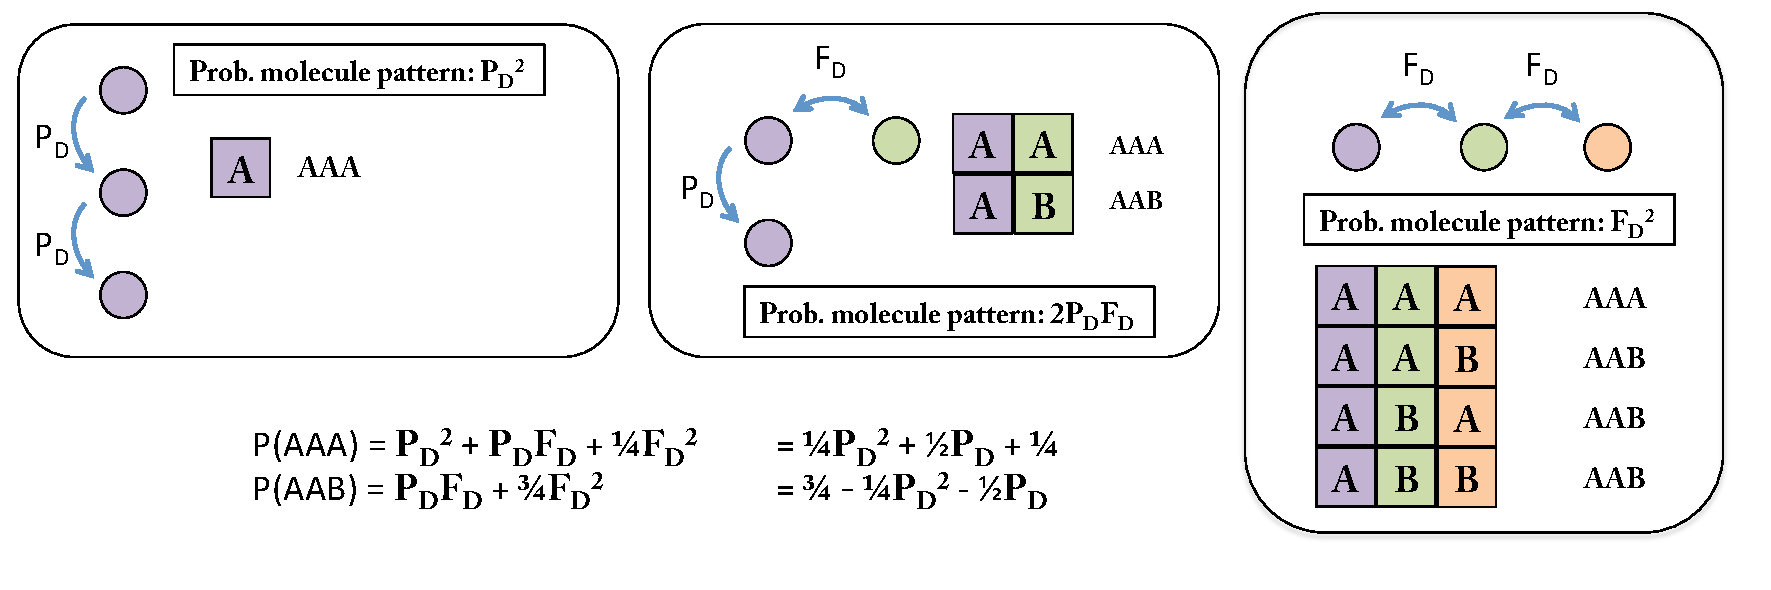
\includegraphics[width=\textwidth]{SuppFigM3.pdf}
\end{center}
\caption{Details of the case when $M=3$.
}
\label{M3example}
\end{figure*}


The log-likelihood is then given as
\begin{equation}
l_3(P_D) = n_{AAA} \log(P(AAA \mid P_D)) + n_{AAB} \log(P(AAB \mid P_D)). 
\end{equation}
\noindent Since this is of the form 
\begin{equation}
l = n \log f(P_D) + m \log (1-f(P_D)),
\end{equation}
\noindent we can see that the first derivative is of the form 
\begin{equation}
n f'(P_D) - (n+m)f'(P_D)f(P_D)
\end{equation}
\noindent So, 
\begin{equation}
\begin{split}
\frac{dl}{dP_D}=&n_{AAA}(\frac{1}{2}P_D+\frac{1}{2}) - \\&(n_{AAA}+n_{AAB})(\frac{1}{2}P_D+\frac{1}{2})(\frac{1}{4}P_D^2+\frac{1}{2}P_D+\frac{1}{4})
\end{split}
\end{equation}
\noindent and since $P_D$ cannot equal $-1$, we have 
\begin{equation}
0 = \hat{P}_D^2 + 2\hat{P}_D + 1 -\frac{4n_{AAA}}{n_{AAA}+n_{AAB}}
\end{equation}
\noindent and
\begin{equation} \label{eq:M3}
\hat{P}_D = -1 \pm 2\sqrt{\frac{n_{AAA}}{n_{AAA}+n_{AAB}}}
\end{equation}

From Figure \ref{M3example}, we can see that for a large numbers of trios, $N = n_{AAA} + n_{AAB}$, $n_{AAA}$ will be approximately equal to $N (\frac{1}{4}P_D^2+\frac{1}{2}P_D+\frac{1}{4})$, which if substituted into the equation for $\hat{P}_D$ gives the estimate $\hat{P}_D = P_D$.

\subsection{Inconsistency with a naive approach when M=3}

Were we to adopt a naive approach, we might simply deal with cases where $M > 2$ by discarding all but 2 fragments in the set at random.

If $M=3$ we would expect to see 

\begin{align}
n_{AA} &= n_{AAA}+\frac{1}{3}n_{AAB}\\
n_{AB} &= \frac{2}{3}n_{AAB}
\end{align}

and so the estimate of $P_D$ will be 

\begin{equation}
\hat{P}_D = 1 - \frac{4n_{AAB}}{3N}
\end{equation}

which in general will not equal the estimate obtained from using all of the data (equation \ref{eq:M3}).
\clearpage{}

\section{Simulation}
% !Rnw root = duplicatessweave.Rnw

\subsection{Artificial data}

We can demonstrate the performance of the method using four artificial data sets that implememnt some of the results just seen

\begin{table}[ht]
\centering
\begin{tabular}{rrrrrrrrr}
  \hline
 & NoSNPs & NoReads & NoDups & AA & AB & AAA & AAB & NoN \\ 
  \hline
Test1 & 1000.00 & 80000.00 & 4000.00 & 2700.00 & 300.00 & 0.00 & 0.00 & 0.00 \\ 
  Test2 & 1000.00 & 80000.00 & 4000.00 & 3800.00 & 200.00 & 0.00 & 0.00 & 0.00 \\ 
  Test3 & 1000.00 & 80000.00 & 4000.00 & 0.00 & 0.00 & 1728.00 & 147.00 & 0.00 \\ 
  Test4 & 1000.00 & 80000.00 & 4000.00 & 1777.00 & 98.00 & 0.00 & 0.00 & 0.00 \\ 
   \hline
\end{tabular}
\end{table}

Test 1 is an $M=2$ case, engineered to have a fragmentation duplicate fraction of $2 \times 300/3000 = 0.2$. \\\\ Test 2 is an $M=2$ case engineered to have a fragmentation duplicate fraction of $2 \times 200/4000 = 0.1$. \\\\ Test 3 is an $M=3$ case engineered to have a fragmentation duplicate fraction of $1- 2 \times \sqrt \frac{1728}{1728+147} = 0.08$.\\\\ Test 4 is the same case using a naive down-sampling to $M=2$ (i.e. one third of AABs end up as AA, the rest as AB). Following the results of the previous section, we do not expect this to return the correct value.

We now read in this table. Then, to prepare for the probability calculations, we  generate the list of sets of partitions possible with each value of $M$ (the number of fragments in a duplicate set). 

\begin{Schunk}
\begin{Sinput}
> HSTtest<-read.delim(paste(EDpath,"/HSTtest.tsv",sep="",collapse=""),header=T,as.is=T)
> PL<-genPL(10)
> CL<-genCoefs(PL)
> processduptable(HSTtest,PL,CL)
\end{Sinput}
\begin{Soutput}
  ObservedDupRate PropFragDups AdjustedDupRate FragDupRate
1               5        0.200           4.000       1.000
2               5        0.100           4.500       0.500
3               5        0.080           4.600       0.400
4               5        0.105           4.475       0.525
\end{Soutput}
\end{Schunk}

We see that after applying the \Rfunction{processduptable} to this artificial data set, the method produces the correct solution in each case.


\subsection{Insert Size Distributions}
To demonstrate that the approach works in a controlled scenario, we use data simulated from the following assumptions: 

\begin{itemize}
\item Read start sites are uniformly distributed along a genome
\item Insert size distributions are sampled from real data independently of the start sites
\item PCR duplicate numbers for each individual read are IID Poisson distributed
\end{itemize}

The size selection step is crucial to the chances of seeing a fragmentation duplicate. Comparing two extreme insert size distributions from our example data set, we can see that (in the absence of any dependence on starting position etc.) the probability of two fragments sampled from the library being the same length differs by a factor of approximately $2.7$ ($0.020$ vs $0.007$).


\begin{Schunk}
\begin{Sinput}
> ISDnarrow<-read.delim(paste(EDpath,"/ISDs/SS6003110.insertsizedist.txt",sep="",collapse=""), as.is=T, header=F)
> ISDwide<-read.delim(paste(EDpath,"/ISDs/SS6003304.insertsizedist.txt",sep="",collapse=""), as.is=T, header=F)
> ISDnarrow<-ISDnarrow[-1000,]
> ISDwide<-ISDwide[-1000,]
> set.seed(31415927)
> table(sample(ISDnarrow[,1], 100000, prob=ISDnarrow[,2], replace=T) == sample(ISDnarrow[,1], 100000, prob=ISDnarrow[,2], replace=T))/100000
\end{Sinput}
\begin{Soutput}
  FALSE    TRUE 
0.97986 0.02014 
\end{Soutput}
\begin{Sinput}
> table(sample(ISDwide[,1], 100000, prob=ISDwide[,2], replace=T) == sample(ISDwide[,1], 100000, prob=ISDwide[,2], replace=T))/100000
\end{Sinput}
\begin{Soutput}
  FALSE    TRUE 
0.99255 0.00745 
\end{Soutput}
\end{Schunk}

Details of the samples that give rise to these distributions are given in Section~\ref{sec:SampInfo}, but it should be noted that the starting tissues and consequently the nucleic acid preparation methods were different. Figure~\ref{duplicatessweave-ISDexplore} illustrates the difference in distributions.

\begin{Schunk}
\begin{Sinput}
> plot(ISDnarrow[,1],ISDnarrow[,2]/sum(ISDnarrow[,2]),xlim=c(200,500),xlab="Insert size",ylab="Density",type="l",lwd=3)
> points(ISDwide[,1],ISDwide[,2]/sum(ISDwide[,2]),col="red",type="l",lwd=3)
> text(375,0.025,"SS6003110")
> text(400,0.01,"SS6003304",col="red")
\end{Sinput}
\end{Schunk}

\incfig[h!]{duplicatessweave-ISDexplore}{\textwidth}{ISDs.}{Examples of extreme insert size distributions.}

If we simulate from these two distributions, we see the effect they have on the fragmentation duplicate proportion.

\begin{Schunk}
\begin{Sinput}
> set.seed(978342)
> HSTsim0<-simreads(depth=60,pcrdup=0.06,realISD=ISDnarrow,lowerlength=0,upperlength=1000,maxM=5)
> HSTsim0<-rbind(HSTsim0,simreads(depth=60,pcrdup=0.06,realISD=ISDwide,lowerlength=0,upperlength=1000,maxM=5))
> PDTsim0<-processduptable(HSTsim0,PL,CL)
> PDTsim0
\end{Sinput}
\begin{Soutput}
     ObservedDupRate PropFragDups AdjustedDupRate FragDupRate
[1,]        6.190174        0.048        5.893046   0.2971284
[2,]        6.195532        0.018        6.084013   0.1115196
\end{Soutput}
\end{Schunk}

We see that the proportion of fragmentation duplicates is substantially lower when using the wider insert size distribution. With the ratio of fragmentation driven duplicate rates also being approximately $2.7$.

\subsection{Demonstration that the method works}

We simulate 1000 heterozygous SNPs, spaced at kilobase intervals. {PCR} duplication rates increase approximately linearly with depth, so we set them accordingly. 

\begin{Schunk}
\begin{Sinput}
> set.seed(62536231)
> HSTsim<-simreads(genlength=1000000,depth=20,pcrdup=0.02,realISD=ISDnarrow,lowerlength=0,upperlength=1000,maxM=5)
> HSTsim<-rbind(HSTsim,simreads(genlength=1000000,depth=40,pcrdup=0.04,realISD=ISDnarrow,lowerlength=0,upperlength=1000,maxM=5))
> HSTsim<-rbind(HSTsim,simreads(genlength=1000000,depth=60,pcrdup=0.06,realISD=ISDnarrow,lowerlength=0,upperlength=1000,maxM=5))
> HSTsim<-rbind(HSTsim,simreads(genlength=1000000,depth=80,pcrdup=0.08,realISD=ISDnarrow,lowerlength=0,upperlength=1000,maxM=5))
> HSTsim<-rbind(HSTsim,simreads(genlength=1000000,depth=100,pcrdup=0.1,realISD=ISDnarrow,lowerlength=0,upperlength=1000,maxM=5))
> PDTsim<-processduptable(HSTsim,PL,CL)
> PDTsim
\end{Sinput}
\begin{Soutput}
     ObservedDupRate PropFragDups AdjustedDupRate FragDupRate
[1,]        2.208724        0.055        2.087245   0.1214798
[2,]        4.250408        0.059        3.999634   0.2507741
[3,]        6.271941        0.045        5.989704   0.2822373
[4,]        8.365719        0.040        8.031091   0.3346288
[5,]       10.354593        0.041        9.930054   0.4245383
\end{Soutput}
\end{Schunk}

\begin{Schunk}
\begin{Sinput}
> plot(seq(20,100,20),PDTsim[,1]/seq(2,10,2),ylim=c(0.95,1.15),xlab="Simulated depth of sequencing",ylab="Estimate/True value",pch=16,main="Using 1000 heterozygous loci")
> abline(h=1,lwd=3)
> points(seq(20,100,20),PDTsim[,3]/seq(2,10,2),col="red",pch=16)
> legend("topright",fill=c("black","red"),legend=c("Observed","Corrected"))
\end{Sinput}
\end{Schunk}

\incfig[h!]{duplicatessweave-Demonstration}{\textwidth}{Performance by depth}{Using 1000 loci, the performance across a range of depths is plotted.}

In figure~\ref{duplicatessweave-Demonstration}, we see that, while there is naturally some stochasticity at low depth (where only 440 duplicate reads are observed), the corrected rate is notably closer (and indeed close) to the true value.

We won't run the following code, as it takes too long for the sweave, but the greater depth emphasizes the improvement even more.

\begin{Schunk}
\begin{Sinput}
> set.seed(3502349)
> HSTsim2<-simreads(depth=200,pcrdup=0.2,realISD=ISDnarrow,lowerlength=0,upperlength=1000)
> #     NoSNPs NoReads NoDups    AA  AB  AAA AAB AAAA AAAB AABB AAAAA AAAAB AAABB AAAAAA AAAAAB AAAABB AAABBB NoN
> #[1,]    999  198406  40725 30693 323 3925 174  410   23   18    33     2     2      1      1      0      0   0
> processduptable(HSTsim2,PL,CL)
> #     ObservedDupRate PropFragDups AdjustedDupRate FragDupRate
> #[1,]        20.52609        0.027        19.97189   0.5542045
\end{Sinput}
\end{Schunk}

\subsection{How many SNPs are required?}

We look now at the effect of changing the number of SNPs being used, for what are otherwise a typical set of parameters. We see that there is some volatility (especially at low values of SNPs), but that even at 500 SNPs the approach is useful. The estimate of the proportion of fragmentation duplicates is quite stable by the time 1000 SNPs are used.

\begin{Schunk}
\begin{Sinput}
> set.seed(5417583)
> HSTsim3<-simreads(genlength=100000,depth=60,pcrdup=0.06,realISD=ISDnarrow,lowerlength=0,upperlength=1000,maxM=6)
> HSTsim3<-rbind(HSTsim3,simreads(genlength=200000,depth=60,pcrdup=0.06,realISD=ISDnarrow,lowerlength=0,upperlength=1000,maxM=6))
> HSTsim3<-rbind(HSTsim3,simreads(genlength=300000,depth=60,pcrdup=0.06,realISD=ISDnarrow,lowerlength=0,upperlength=1000,maxM=6))
> HSTsim3<-rbind(HSTsim3,simreads(genlength=400000,depth=60,pcrdup=0.06,realISD=ISDnarrow,lowerlength=0,upperlength=1000,maxM=6))
> HSTsim3<-rbind(HSTsim3,simreads(genlength=500000,depth=60,pcrdup=0.06,realISD=ISDnarrow,lowerlength=0,upperlength=1000,maxM=6))
> HSTsim3<-rbind(HSTsim3,simreads(genlength=750000,depth=60,pcrdup=0.06,realISD=ISDnarrow,lowerlength=0,upperlength=1000,maxM=6))
> HSTsim3<-rbind(HSTsim3,simreads(genlength=1000000,depth=60,pcrdup=0.06,realISD=ISDnarrow,lowerlength=0,upperlength=1000,maxM=6))
> HSTsim3<-rbind(HSTsim3,simreads(genlength=1500000,depth=60,pcrdup=0.06,realISD=ISDnarrow,lowerlength=0,upperlength=1000,maxM=6))
> HSTsim3<-rbind(HSTsim3,simreads(genlength=2000000,depth=60,pcrdup=0.06,realISD=ISDnarrow,lowerlength=0,upperlength=1000,maxM=6))
> PDTsim3<-processduptable(HSTsim3,PL,CL)
> PDTsim3
\end{Sinput}
\begin{Soutput}
      ObservedDupRate PropFragDups AdjustedDupRate FragDupRate
 [1,]        5.735913        0.053        5.431909   0.3040034
 [2,]        6.015038        0.031        5.828571   0.1864662
 [3,]        6.576102        0.036        6.339362   0.2367397
 [4,]        6.238972        0.047        5.945740   0.2932317
 [5,]        6.232533        0.053        5.902209   0.3303243
 [6,]        6.345920        0.053        6.009586   0.3363338
 [7,]        6.159110        0.050        5.851155   0.3079555
 [8,]        6.185923        0.043        5.919928   0.2659947
 [9,]        6.328509        0.041        6.069040   0.2594689
\end{Soutput}
\end{Schunk}

Plotting the performance of the method with differing numbers of SNPs we see that anything more than 500 heterozygous loci should suffice for a typical depth of sequencing (Figure~\ref{duplicatessweave-SNPnumberplot}).

\begin{Schunk}
\begin{Sinput}
> plot(HSTsim3[,1],PDTsim3[,1],ylim=c(5,7),,xlim=c(0,2000),pch=16,xlab="Number of Heterozygous SNPs used",ylab="Estimates (percentage)",main="True value = 6",type="b",lwd=2)
> points(HSTsim3[,1],PDTsim3[,3],pch=16,col="red",type="b",lwd=2)
> legend("topright",fill=c("black","red"),legend=c("Observed","Corrected"))
> abline(h=6,lwd=3)
\end{Sinput}
\end{Schunk}

\incfig[h!]{duplicatessweave-SNPnumberplot}{\textwidth}{SNP numbers}{We see that at this (typical) depth, the performance of the method becomes stable once 400 SNPs have been used.}

The suggestion from the previous two sections is that approximately 1500 duplicate reads are required (whether arising through high depth or a high number of heterozygoius loci).
\clearpage{}

\section{SNPs to extract}
\label{sec:SNPs}
% !Rnw root = duplicatessweave.Rnw

\subsection{Choosing the SNPs}

We investigate $2,500$ common SNPs in anticipation of identifying $1,000$ heterozygous sites for each sample. In this manner we avoid the burden of having to define a bespoke set of sites for each case.

The SNPs were selected from UCSC's snp138Common table, considering only those validated by the $1000$ Genomes Project. We required the reported population minor allele frequency (MAF) of selected SNPs be $>0.49$ based on $>2,500$ observations and that the SNPs were located on one of the $24$ `regular' chromosomes. The $2,500$  SNPs were selected at random from all those meeting the criteria. 

Despite these criteria, the true MAF can only be biased in one direction from the approximately $0.5$ we nominally required, and our sequencing depth and requirements for calling heterozygous SNPs in the data mean that we will fail to identify up to ten percent of heterozygous sites because, by chance, their observed allele frequencies will be too extreme. Additionally, $35$ of the randomly selected SNPs were from the sex chromosomes, and are `unlikely' to be heterozygous in our predominantly male patients. In combination, these effects mean that we can anticipate approximately $1,000$ of the SNPs to be heterozygous in each patient.

By choosing a set of SNPs with high MAF, we can guarantee a good number of heterozygous observations in each sample, without the computational burden of defining a bespoke set of sites for each case. Extracting all reads mapping to these locations creates a BAM file that is approximately $10,000$ times smaller than the original and so allows for easy manipulation of large cohorts. We note that such a set of SNPs, and the BAM file they produce, are also useful for activities such as i) detecting sample contamination, ii) detecting sample mix ups, iii) detecting familial/ancestral relationships, and so have utility beyond our purposes in this study.

We now load in the set of SNPs and explore them.

\begin{Schunk}
\begin{Sinput}
> snplist<-read.delim(file.path(EDpath,"SNPstoextract.txt"),as.is=T,header=T)
\end{Sinput}
\end{Schunk}


\subsection{Representativeness of the SNPs}

\subsubsection{Distribution across Chromosomes}
We can see (Figure~\ref{duplicatessweave-AddFig1}) that the SNPs are chosen from all chromosomes (Figure \ref{duplicatessweave-AddFig1}), and that we are not far from having numbers proportional to chromosome length.

\begin{Schunk}
\begin{Sinput}
> par(mar=c(4.6,4.1,1.6,1.6))
> plot(table(snplist$chrom)[c(1,12,16:22,2:11,13:15,23:24)], 
+      ylab="number of SNPs",xlab="chromosome",axes=F)
> axis(2)
> axis(1,labels=c(1:22,"X","Y"),at=1:24,las=2)
> box()
\end{Sinput}
\end{Schunk}

\incfig[h]{duplicatessweave-AddFig1}{\textwidth}{SNP numbers.}
{The numbers of SNPs used from each chromosome.}

\subsubsection{GC content}

We take the locations of the $2,500$ SNPs in our list and place a window of $500$ bases around them, before counting the number of G and C bases in that window.

\begin{Schunk}
\begin{Sinput}
> genome <- Hsapiens
> GCNo<-rep(NA,2500)
> for(i in 1:2500){
+   GCNo[i]<-sum(unlist(strsplit(as.character(substr(genome[[snplist$chrom[i]]],snplist$chromEnd[i]-250,snplist$chromEnd[i]+249)),"")) %in% c("G","C"))
+ }
\end{Sinput}
\end{Schunk}

For comparison, we take the human genome (chromosomes 1-22 and X), divide it up into bins of $500$ and calculate the proportion of bases that are G or C in each bin.


\begin{Schunk}
\begin{Sinput}
> GCbinned<-NULL
> for(k in 1:23){
+     windowViews <- trim(Views(genome[[k]], start = seq(1, length(genome[[k]]), 500), width = 500))
+     letterFreq <- letterFrequency(windowViews, letters = c("A","C","G","T"))
+     seqGC <- rowSums(letterFreq[,2:3]) / rowSums(letterFreq)
+     GCbinned<-c(GCbinned,seqGC)
+ }
\end{Sinput}
\end{Schunk}

We see (Figure~\ref{duplicatessweave-AddFigSNPGC}) that the distribution of GC in our selection is a good representation of the GC content of the genome (with departure only in the final percentile).


\begin{Schunk}
\begin{Sinput}
> par(mfrow=c(1,2))
> hist(GCbinned,freq=F,col=rgb(1,0.5,0.5,0.5),breaks=seq(0,1,0.02),main="Distribution of GC content of genome",xlab="GC proportion")
> hist(GCNo/500,freq=F,col=rgb(0.5,0.5,1,0.5),breaks=seq(0,1,0.02),add=T)
> legend("topright",fill=c(rgb(1,0.5,0.5,0.5),rgb(0.5,0.5,1,0.5)),legend=c("Genome-wide","Our SNPs"))
> plot(quantile(GCbinned,probs=seq(0.01,.99,0.01),na.rm=T),quantile(GCNo/500,probs=seq(.01,.99,0.01),na.rm=T),
+      pch=20,col="red",xlab="Genome wide 1st - 99th percentiles",
+      ylab="Our SNPs 1st - 99th percentiles",
+      main="Proportion GC Content\nKolmogorov-Smirnov p=0.08")
> for(i in 1:99){
+   GW<-quantile(GCbinned,probs=i/100,na.rm=T)
+   OS<-quantile(GCNo/500,probs=i/100,na.rm=T)
+ lines(c(GW,GW),c(0,OS),lwd=0.5)  
+ lines(c(0,GW),c(OS,OS),lwd=0.5)  
+ }
> points(quantile(GCbinned,probs=seq(0.01,.99,0.01),na.rm=T),quantile(GCNo/500,probs=seq(.01,.99,0.01),na.rm=T),pch=20,col="red")
> abline(0,1,lwd=2)
\end{Sinput}
\end{Schunk}
\incfig[h]{duplicatessweave-AddFigSNPGC}{\textwidth}{SNP GC representativeness.}
{Illustrating that the distribution of GC in our selection is a good representation of the GC content of the genome.}

Despite the power to detect deviation with this number of samples, the Kolmogorov-Smirnov test is not significant.

\begin{Schunk}
\begin{Sinput}
> ks.test(GCbinned,GCNo/500)
\end{Sinput}
\begin{Soutput}
	Two-sample Kolmogorov-Smirnov test

data:  GCbinned and GCNo/500
D = 0.02552, p-value = 0.07717
alternative hypothesis: two-sided
\end{Soutput}
\end{Schunk}



\clearpage{}


\section{Sample information}
\label{sec:SampInfo}
% !Rnw root = duplicatessweave.Rnw



We are considering twenty-two `normal' samples from patients forming part of the \href{http://www.compbio.group.cam.ac.uk/research/icgc}{Oesophageal Adenocarcinoma ICGC} study run by the \href{http://www.mrc-cu.cam.ac.uk/our\_research/Rebecca\_Fitzgerald/occams.html}{OCCAMS Consortium}. The full data for these samples are archived in the European Genome Archive [\href{https://www.ebi.ac.uk/ega/datasets/EGAD00001000704}{EGA:EGAD00001000704}] and have featured in the paper \href{http://www.nature.com/ng/journal/v46/n8/abs/ng.3013.html}{Ordering of mutations in preinvasive disease stages of esophageal carcinogenesis}. 

Of the twenty-two samples, twelve were blood, and ten were oesophageal tissue. DNA from oesophageal tissue was extracted using the DNeasy kit (Qiagen) and from blood using the NucleonTM Genomic Extraction kit (Gen-Probe) (according to the manufacturer's instructions). 

The sequencing was conducted under contract by Illumina, typically comprising five lanes of 100bp paired end sequencing. The depth of coverage ranges from $57$x to $87$x with a mean of $68$x.

In addition, we use one tumour sample from the same study. 

This study is a presentation of analysis methods not a presentation of the sequencing data, and raw data that could identify the patients is not provided. Sufficient data are provided to illustrate the methods presented. Further access is via the Project's Data Access Committee. 



\subsection{Picard}

Picard was applied to the raw bam files, and from this output we extract data on the number of read pairs examined, the numbers of read pairs marked as duplicates, and the number of read pairs marked as optical duplicates. We keep the full results for incorporation into Table 1.


\begin{Schunk}
\begin{Sinput}
> unmaskedP<-read.delim(file.path(EDpath,"Picard", "samples.metrics.txt"),as.is=T)
> readPairsExamined <- readPairDuplicates <- OpticalPairDuplicates <- matrix(ncol=9, nrow=22, dimnames = list(unmaskedP[,1], c("Total", "X", "Y", "M", "Centromeres", "Telomeres", "LowCov", "HighCov", "Residual")))
> readPairsExamined[,1]<-unmaskedP[,3]
> readPairDuplicates[,1]<-unmaskedP[,6]
> OpticalPairDuplicates[,1]<-unmaskedP[,7]
\end{Sinput}
\end{Schunk}


\subsubsection{Generate Table 1}

We read in supplementary table 1 from Weaver et al, and extract the information of interest to us.

\begin{Schunk}
\begin{Sinput}
> WeaverSuppTable1<-read.delim(file.path(EDpath,"WeaverSuppTable1.txt"),sep="",header=T,as.is=T)
> WeaverSuppTable1$CaseID<-WeaverSuppTable1$CaseID-1
\end{Sinput}
\end{Schunk}

Next we collect the information for Table 1 of the main manuscript, and prepare it for insertion into the LaTeX document.

\begin{Schunk}
\begin{Sinput}
> Table1<-cbind(WeaverSuppTable1[,1],WeaverSuppTable1[,2],WeaverSuppTable1[,12],round(unmaskedP[,3]/1000000000,2),round(100*unmaskedP[,6]/unmaskedP[,3],2),round(unmaskedP[,9]/1000000000,2))
> Table1[Table1=="NormalOesophagus"]<-"NormalOes"
> colnames(Table1)<-c("ID","Sex","Tissue","Reads (10^9)","Dup. Rate (%)","Library Size (10^9)")
> xtab1<-xtable(Table1)
> write(print(xtab1,include.rownames = FALSE),file="Table1.txt")
\end{Sinput}
% latex table generated in R 3.2.3 by xtable 1.8-2 package
% Tue Mar 29 21:22:37 2016
\begin{table}[ht]
\centering
\begin{tabular}{llllll}
  \hline
ID & Sex & Tissue & Reads (10\verb|^|9) & Dup. Rate (\%) & Library Size (10\verb|^|9) \\ 
  \hline
3108 & Female & Blood & 1.15 & 6.15 & 9.03 \\ 
  3110 & Male & Blood & 1.16 & 7.86 & 7 \\ 
  3112 & Male & Blood & 1.29 & 6.94 & 8.86 \\ 
  3114 & Male & Blood & 0.88 & 5.05 & 8.46 \\ 
  3116 & Male & NormalOes & 0.93 & 11.92 & 3.59 \\ 
  3118 & Male & NormalOes & 1.16 & 14.49 & 3.61 \\ 
  3120 & Male & Blood & 1.11 & 4.01 & 13.55 \\ 
  3124 & Male & Blood & 0.99 & 8.07 & 5.81 \\ 
  3128 & Male & Blood & 0.97 & 4.8 & 9.8 \\ 
  3130 & Male & Blood & 1.03 & 8.34 & 5.83 \\ 
  3132 & Male & Blood & 1.02 & 6.03 & 8.15 \\ 
  3134 & Male & Blood & 1.1 & 4.38 & 12.21 \\ 
  3136 & Male & Blood & 0.99 & 5.76 & 8.3 \\ 
  3148 & Female & Blood & 1.03 & 3.73 & 13.55 \\ 
  3301 & Male & NormalOes & 0.89 & 5.92 & 7.27 \\ 
  3304 & Male & NormalOes & 1.01 & 8.37 & 5.74 \\ 
  3307 & Male & NormalOes & 1.04 & 6.85 & 7.27 \\ 
  3310 & Female & NormalOes & 1.03 & 10.71 & 4.46 \\ 
  3313 & Female & NormalOes & 1 & 5.22 & 9.31 \\ 
  3316 & Male & NormalOes & 0.97 & 5.99 & 7.86 \\ 
  3319 & Male & NormalOes & 1.05 & 8.24 & 6.01 \\ 
  3322 & Male & NormalOes & 0.93 & 11.34 & 3.8 \\ 
   \hline
\end{tabular}
\end{table}\end{Schunk}

We will define four groups based on sex and the origin of the tissue/DNA extraction kit used.

\begin{Schunk}
\begin{Sinput}
> table(WeaverSuppTable1[,2],WeaverSuppTable1[,12])
\end{Sinput}
\begin{Soutput}
         Blood NormalOesophagus
  Female     2                2
  Male      10                8
\end{Soutput}
\begin{Sinput}
> Group<-1+2*(WeaverSuppTable1[,2]=="Male")+(WeaverSuppTable1[,12]=="Blood")
> GroupN<-c("Female_Tissue","Female_Blood","Male_Tissue","Male_Blood")[Group]
\end{Sinput}
\end{Schunk}

\subsubsection{Masks}

The proportion of duplicate reads that are due to coincidental fragmentation is not constant along the genome due to changes in copy number and mapping accuracy. We attempt to restrict ourselves to regions where this proportion will be constant by masking areas that are likely to be problematic. The regions that we mask out of the genome for this study are defined in the \file{.bed} files in this package. For instance, the Centromeres are masked out by the 4th mask file. For further reference, we will record the total genome size, sizes of masked regions, and the remainder (residual).

\begin{Schunk}
\begin{Sinput}
> list.files(file.path(EDpath,"masks"))
\end{Sinput}
\begin{Soutput}
[1] "Mask1-ChrX.bed"        "Mask2-ChrY.bed"        "Mask3-ChrM.bed"       
[4] "Mask4-Centromeres.bed" "Mask5-Telomeres.bed"   "Mask6-lowdepth.bed"   
[7] "Mask7-highdepth.bed"  
\end{Soutput}
\begin{Sinput}
> maskFiles <- list.files(file.path(EDpath,"masks"), full.names = TRUE)
> MASKS <- lapply(maskFiles, read.delim, header=FALSE, as.is=TRUE, skip=1)
> effectiveGenomeSize<-rep(0,9)
> effectiveGenomeSize[1]<-sum(as.numeric(MASKS[[5]][17:38,3]))
> +MASKS[[1]][1,3]+MASKS[[2]][1,3]+MASKS[[3]][1,3]
\end{Sinput}
\begin{Soutput}
[1] 214676571
\end{Soutput}
\begin{Sinput}
> for(i in 1:7){ 
+     effectiveGenomeSize[i+1] <- sum(MASKS[[i]][,3] - MASKS[[i]][,2])}
> effectiveGenomeSize[9]<-effectiveGenomeSize[1]-sum(effectiveGenomeSize[2:8])
\end{Sinput}
\end{Schunk}

Note that there is no real penalty for masking too much of the genome, as we have seen that only 1000 heterozygous SNPs are required, which suggests that less than $0.1\%$ of the genome is required.

\subsubsection{Picard Output}

Picard was run on bam files defined by these masks (separately for each mask) and we read these data into the matrices created earlier, before creating Table 2 in the paper.

We only use the "READ\_PAIRS\_EXAMINED", "READ\_PAIR\_DUPLICATES", and "READ\_PAIR\_OPTICAL\_DUPLICATES" values that Picard produces (as indeed does Picard for this problem). For simplicity, we create three tables to take these values and store in them the Picard output for the entire samples, and then also for Picard output generated from the masked regions.

\begin{Schunk}
\begin{Sinput}
> metfiles<-list.files(file.path(EDpath,"Picard"))
> metfiles<-grep("mask",metfiles,value=T)
> for(i in 1:7){
+   temp<-read.delim(file.path(EDpath,"Picard",metfiles[i]),as.is=T)
+   temp<-temp[-(15:19),]
+   readPairsExamined[,i+1]<-temp[,3]
+   readPairDuplicates[,i+1]<-temp[,6]
+   OpticalPairDuplicates[,i+1]<-temp[,7]
+ }
\end{Sinput}
\end{Schunk}

We now calculate the 'residual' counts by subtracting the masked regions from the total.

\begin{Schunk}
\begin{Sinput}
> readPairsExamined[,9]<-readPairsExamined[,1]-apply(readPairsExamined[,2:8],1,sum)
> readPairDuplicates[,9]<-readPairDuplicates[,1]-apply(readPairDuplicates[,2:8],1,sum)
> OpticalPairDuplicates[,9]<-OpticalPairDuplicates[,1]-apply(OpticalPairDuplicates[,2:8],1,sum)
\end{Sinput}
\end{Schunk}


\subsubsection{Generate Table 2}

Now we report the residual values and the numbers for the masked regions relative to the residual values. This is Table 2 of the main manuscript. 

\begin{Schunk}
\begin{Sinput}
> reptable<-matrix(0,ncol=4,nrow=8)
> reptable[1,]<-round(100*sapply(split(((readPairDuplicates[,9]/readPairsExamined[,9])),Group),mean),2)
> for(i in 2:8){
+   reptable[i,]<-round(sapply(split((
+     (readPairDuplicates[,i]/readPairsExamined[,i])
+     /(readPairDuplicates[,9]/readPairsExamined[,9])),Group),mean),2)
+ }
> reptable[3,1:2]<-"-"
> rownames(reptable)<-c("Residual","X","Y","M","Centromeres","Telomeres","Low Cov","High Cov")
> colnames(reptable)<-c("Female Tissue","Female Blood","Male Tissue","Male Blood")
> write(print(xtable(reptable)),file="Table2.txt")
\end{Sinput}
% latex table generated in R 3.2.3 by xtable 1.8-2 package
% Tue Mar 29 21:22:37 2016
\begin{table}[ht]
\centering
\begin{tabular}{rllll}
  \hline
 & Female Tissue & Female Blood & Male Tissue & Male Blood \\ 
  \hline
Residual & 6.82 & 3.48 & 7.8 & 4.43 \\ 
  X & 1.23 & 1.43 & 1.09 & 1.2 \\ 
  Y & - & - & 4.6 & 9.19 \\ 
  M & 7.41 & 14.62 & 5.62 & 5.05 \\ 
  Centromeres & 4.45 & 8.46 & 3.88 & 7.37 \\ 
  Telomeres & 0.99 & 1.19 & 0.98 & 1.09 \\ 
  Low Cov & 0.94 & 0.95 & 0.93 & 0.94 \\ 
  High Cov & 1.6 & 2.76 & 1.44 & 2.45 \\ 
   \hline
\end{tabular}
\end{table}\end{Schunk}


\clearpage{}

\section{SNP numbers in our samples}
% !Rnw root = duplicatessweave.Rnw

\subsection{Processing the SNPs}

The following code will not be evaluated, as the patients' data are not distributed with this sweave, but can be obtained from the European Genome Archive (as previously noted). The summary data which are distributed are loaded in after this section, but the code here shows how they were created.

Later, we are going to contrast the estimate obtained from SNPs in high-GC regions with that from those in low-GC regions. We prepare for this analysis now also.

\begin{Schunk}
\begin{Sinput}
> HetSNPTable<-processBAMfordups(bamfilelist=bamfilelist,path=path,snplist=snplist)
> write.table(HetSNPTable,file="HetSNPDups.txt",sep="\t")
> HetSNPTableLowGC<-processBAMfordups(bamfilelist=bamfilelist,path=path,snplist=snplist[GCNo<199,])
> HetSNPTableHighGC<-processBAMfordups(bamfilelist=bamfilelist,path=path,snplist=snplist[GCNo>=199,])
> write.table(HetSNPTableHighGC,file="HetSNPDupsHighGC.txt",sep="\t") 
> write.table(HetSNPTableLowGC,file="HetSNPDupsLowGC.txt",sep="\t")
\end{Sinput}
\end{Schunk}


\subsection{Exploration of SNP numbers}
\subsubsection{Preliminaries}

We now load in the summary of the numbers of SNPs being investigated, and generate the various results given in the section "SNP numbers and duplicate numbers" in the main manuscript.

\begin{Schunk}
\begin{Sinput}
> HetSNPTable<-read.delim(file.path(EDpath,"HetSNPDups.txt"),as.is=T)
\end{Sinput}
\end{Schunk}

We define the duplicate rate as the number of duplicates identified within the unmasked regions of the genome divided by the number of read-pairs examined within those regions.

\begin{Schunk}
\begin{Sinput}
> ResDupR<-readPairDuplicates[,9]/readPairsExamined[,9]
\end{Sinput}
\end{Schunk}

We define the residual read depth as 200 (the number of bases sequenced per read-pair) multiplied by the number of read-pairs examined, divided by the length of the unmasked genome.

\begin{Schunk}
\begin{Sinput}
> ResDepth<-round(200*readPairsExamined[,9]/effectiveGenomeSize[9],2)
\end{Sinput}
\end{Schunk}

\subsubsection{How many SNPs do we see?}

``From the 2,500 sites considered, the median number of heterozygous SNPs identified per sample is 1,009 (range 942 to 1,093).''

\begin{Schunk}
\begin{Sinput}
> summary(HetSNPTable[,1])
\end{Sinput}
\begin{Soutput}
   Min. 1st Qu.  Median    Mean 3rd Qu.    Max. 
  942.0   988.5  1009.0  1015.0  1034.0  1093.0 
\end{Soutput}
\end{Schunk}

``Average read depth (as measured by the number of reads mapping to the regions of the genome that we are not masking) is correlated with the number of heterozygous SNPs (correlation = 0.52, p = 0.014): a reflection on our stringent calling criterion.''

\begin{Schunk}
\begin{Sinput}
> summary(lm(HetSNPTable[,1]~ResDepth+ResDupR))
\end{Sinput}
\begin{Soutput}
Call:
lm(formula = HetSNPTable[, 1] ~ ResDepth + ResDupR)

Residuals:
    Min      1Q  Median      3Q     Max 
-64.061 -17.787   1.512  25.908  50.541 

Coefficients:
            Estimate Std. Error t value Pr(>|t|)    
(Intercept)  803.774     81.198   9.899  6.2e-09 ***
ResDepth       2.714      1.033   2.627   0.0166 *  
ResDupR       -1.191    262.094  -0.005   0.9964    
---
Signif. codes:  0 ‘***’ 0.001 ‘**’ 0.01 ‘*’ 0.05 ‘.’ 0.1 ‘ ’ 1

Residual standard error: 34.61 on 19 degrees of freedom
Multiple R-squared:  0.2671,	Adjusted R-squared:   0.19 
F-statistic: 3.463 on 2 and 19 DF,  p-value: 0.0522
\end{Soutput}
\begin{Sinput}
> cor.test(ResDepth,HetSNPTable[,1])
\end{Sinput}
\begin{Soutput}
	Pearson's product-moment correlation

data:  ResDepth and HetSNPTable[, 1]
t = 2.7001, df = 20, p-value = 0.01377
alternative hypothesis: true correlation is not equal to 0
95 percent confidence interval:
 0.1217976 0.7705574
sample estimates:
      cor 
0.5168646 
\end{Soutput}
\end{Schunk}

\subsubsection{How many duplicate read pairs are we using?}

``The number of sets of duplicate read fragments observed to overlie the heterozygous SNP sites varies from $1,334$ to $9,513$.''

\begin{Schunk}
\begin{Sinput}
> #summary(apply(HetSNPTable[,-1],1,sum))
> summary(HetSNPTable[,3])
\end{Sinput}
\begin{Soutput}
   Min. 1st Qu.  Median    Mean 3rd Qu.    Max. 
   1334    2483    3442    3768    4709    9513 
\end{Soutput}
\end{Schunk}
``The number of duplicate sets is unsurprisingly dependent on the duplicate rate ($p < 2 x 10^{-16}$) and the depth of coverage ($p = 3.3 x 10^{-5}$), but not directly on the number of heterozygous sites being considered (although this is correlated with the depth of coverage).''

\begin{Schunk}
\begin{Sinput}
> summary(lm(HetSNPTable[,3]~ResDupR+HetSNPTable[,1]+ResDepth))
\end{Sinput}
\begin{Soutput}
Call:
lm(formula = HetSNPTable[, 3] ~ ResDupR + HetSNPTable[, 1] + 
    ResDepth)

Residuals:
    Min      1Q  Median      3Q     Max 
-867.83  -75.79   71.24  130.24  342.18 

Coefficients:
                  Estimate Std. Error t value Pr(>|t|)    
(Intercept)      -7342.603   1515.346  -4.845  0.00013 ***
ResDupR          67071.320   1971.187  34.026  < 2e-16 ***
HetSNPTable[, 1]     3.311      1.725   1.919  0.07096 .  
ResDepth            49.726      9.073   5.481 3.32e-05 ***
---
Signif. codes:  0 ‘***’ 0.001 ‘**’ 0.01 ‘*’ 0.05 ‘.’ 0.1 ‘ ’ 1

Residual standard error: 260.3 on 18 degrees of freedom
Multiple R-squared:  0.9859,	Adjusted R-squared:  0.9835 
F-statistic: 418.2 on 3 and 18 DF,  p-value: < 2.2e-16
\end{Soutput}
\end{Schunk}

\subsubsection{How do the duplicates read pairs break down into pairs, triples, etc.?}

``Of the total of 82,903 sets of duplicate fragments identified among the 22 samples, ...''


\begin{Schunk}
\begin{Sinput}
> sum(HetSNPTable[,3])
\end{Sinput}
\begin{Soutput}
[1] 82903
\end{Soutput}
\end{Schunk}

``...the vast majority (73,767 or 89\%) are duplicate pairs,''

\begin{Schunk}
\begin{Sinput}
> sum(HetSNPTable[,4:5])
\end{Sinput}
\begin{Soutput}
[1] 73767
\end{Soutput}
\begin{Sinput}
> round(100*sum(HetSNPTable[,4:5])/sum(HetSNPTable[,3]))
\end{Sinput}
\begin{Soutput}
[1] 89
\end{Soutput}
\end{Schunk}

``...8,262 (10\%) are triples,...''
\begin{Schunk}
\begin{Sinput}
> sum(2*HetSNPTable[,6:7])
\end{Sinput}
\begin{Soutput}
[1] 8262
\end{Soutput}
\begin{Sinput}
> round(100*2*sum(HetSNPTable[,6:7])/sum(HetSNPTable[,3]))
\end{Sinput}
\begin{Soutput}
[1] 10
\end{Soutput}
\end{Schunk}

``...771 (0.9\%) are quartets,...'' 
\begin{Schunk}
\begin{Sinput}
> sum(3*HetSNPTable[,8:10])
\end{Sinput}
\begin{Soutput}
[1] 771
\end{Soutput}
\begin{Sinput}
> round(100*3*sum(HetSNPTable[,8:10])/sum(HetSNPTable[,3]))
\end{Sinput}
\begin{Soutput}
[1] 1
\end{Soutput}
\end{Schunk}

``and the greatest number of fragments seen in a duplicate set is six (one instance).''
\begin{Schunk}
\begin{Sinput}
> sum(HetSNPTable[,14:17])
\end{Sinput}
\begin{Soutput}
[1] 1
\end{Soutput}
\end{Schunk}

\clearpage{}

\section{Duplicate rate estimates}
\label{sec:Estimates}
% !Rnw root = duplicatessweave.Rnw

\subsection{Estimating the fragmentation-duplicate proportion}


We now calculate the maximum likelihood estimates of the proportions of duplicates that are fragmentation duplicates.

\begin{Schunk}
\begin{Sinput}
> PL<-genPL(16)
> CL<-genCoefs(PL)
> FDres<-processduptable(HetSNPTable,PL,CL)
> FDres
\end{Sinput}
\begin{Soutput}
              ObservedDupRate PropFragDups AdjustedDupRate FragDupRate
SS6003108.bam        4.072517        0.086        3.722281   0.3502365
SS6003110.bam        5.577882        0.082        5.120496   0.4573864
SS6003112.bam        4.634298        0.098        4.180136   0.4541612
SS6003114.bam        2.602954        0.093        2.360879   0.2420747
SS6003116.bam        9.250972        0.036        8.917937   0.3330350
SS6003118.bam       12.130834        0.033       11.730516   0.4003175
SS6003120.bam        1.922691        0.198        1.541998   0.3806928
SS6003124.bam        5.917578        0.065        5.532936   0.3846426
SS6003128.bam        2.274395        0.160        1.910492   0.3639032
SS6003130.bam        6.170018        0.058        5.812157   0.3578610
SS6003132.bam        3.889274        0.072        3.609246   0.2800277
SS6003134.bam        2.071006        0.176        1.706509   0.3644970
SS6003136.bam        3.661727        0.094        3.317525   0.3442024
SS6003148.bam        1.853215        0.170        1.538169   0.3150466
SS6003301.bam        4.169853        0.042        3.994719   0.1751338
SS6003304.bam        6.814179        0.017        6.698338   0.1158410
SS6003307.bam        5.181666        0.039        4.979581   0.2020850
SS6003310.bam        8.962766        0.039        8.613218   0.3495479
SS6003313.bam        3.683735        0.060        3.462711   0.2210241
SS6003316.bam        4.271865        0.033        4.130893   0.1409715
SS6003319.bam        6.301027        0.098        5.683526   0.6175006
SS6003322.bam        9.855291        0.019        9.668041   0.1872505
\end{Soutput}
\end{Schunk}

\subsection{The Picard estimates}

From Picard, we generate two estimates of the duplication rate: the basic estimate as reported by Picard and a residual estimate generated only from regions of the genome that are not masked. 

\begin{Schunk}
\begin{Sinput}
>   BasicEst<-(readPairDuplicates[,1]-OpticalPairDuplicates[,1])/
+   (readPairsExamined[,1]-OpticalPairDuplicates[,1])
>   ResidEst<-(readPairDuplicates[,9]-OpticalPairDuplicates[,9])/
+   (readPairsExamined[,9]-OpticalPairDuplicates[,9])
\end{Sinput}
\end{Schunk}


We now generate Figure 2 from the main manuscript (Figure \ref{duplicatessweave-AddFig2} in this document).

\begin{Schunk}
\begin{Sinput}
>   par(mfrow=c(1,2))
> plot(c(0,0.15),c(0,0.15),type="n",xlab="Estimates from 2,500 SNPs",ylab="Picard Estimates",main="Uncorrected Estimates")
> for(i in 1:22){
+ lines(c(FDres[i,1]/100,FDres[i,1]/100),c(BasicEst[i],ResidEst[i]))
+ points(FDres[i,1]/100,BasicEst[i],pch=16,col="red")
+ points(FDres[i,1]/100,ResidEst[i],pch=16,col="black")
+ }
> abline(0,1)
> legend("bottomright",fill=c("red","black"),legend=c("Basic Estimate","Masked Estimate"))
> plot(100*BasicEst/FDres[,3],FDres[,1]/FDres[,3],xlim=c(0.9,2.6),ylim=c(0.9,1.3),pch=16,xlab="Picard Estimate/Corrected Estimate",ylab="Observation from SNPs/Corrected Estimate",main="PCR duplicate rate")
> abline(v=1,lwd=2)
> abline(h=1,lwd=2)
\end{Sinput}
\end{Schunk}

\incfig[ht!]{duplicatessweave-AddFig2}{\textwidth}{The different estimates of duplication rate}

We see in Figure~\ref{duplicatessweave-AddFig2} that the masking of regions of the genome does a good job, but consistently fails to bring the estimate of the overall duplicate rate down to that observed from the 2,500 loci. Thus we use our observed duplicate rate from the SNPs as our baseline, and see that after correction it is reduced by up to one fifth. The original (standard) Picard estimate can overestimate the rate by a factor of 2.5.

\subsection{Other properties}

How many more reads are being marked as duplicates than we would want?

\begin{Schunk}
\begin{Sinput}
> readPairDuplicates[,1]-(FDres[,3]/100)*readPairsExamined[,1]/(1+FDres[,3]/100)
\end{Sinput}
\begin{Soutput}
SS6003108 SS6003110 SS6003112 SS6003114 SS6003116 SS6003118 SS6003120 SS6003124 SS6003128 
 29524695  34627752  37656006  24215186  34653344  46385765  27703407  28002007  28282071 
SS6003130 SS6003132 SS6003134 SS6003136 SS6003148 SS6003301 SS6003304 SS6003307 SS6003310 
 29212616  25963937  29626744  25286539  22808089  18449851  21152158  21947459  28546788 
SS6003313 SS6003316 SS6003319 SS6003322 
 18793636  19561578  29921162  23449747 
\end{Soutput}
\end{Schunk}

What depth of coverage does this represent?

\begin{Schunk}
\begin{Sinput}
> round((readPairDuplicates[,1]-(FDres[,3]/100)*readPairsExamined[,1]/(1+FDres[,3]/100))*200/effectiveGenomeSize[1],1)
\end{Sinput}
\begin{Soutput}
SS6003108 SS6003110 SS6003112 SS6003114 SS6003116 SS6003118 SS6003120 SS6003124 SS6003128 
      2.0       2.4       2.6       1.7       2.4       3.2       1.9       1.9       2.0 
SS6003130 SS6003132 SS6003134 SS6003136 SS6003148 SS6003301 SS6003304 SS6003307 SS6003310 
      2.0       1.8       2.1       1.8       1.6       1.3       1.5       1.5       2.0 
SS6003313 SS6003316 SS6003319 SS6003322 
      1.3       1.4       2.1       1.6 
\end{Soutput}
\end{Schunk}
\clearpage{}

\section{Observations on consistency}
% !Rnw root = duplicatessweave.Rnw

\subsection{Agreement of estimate from M equal to 2, with estimate from M greater than 2}

We can separate out the estimate when $M=2$ from that when $M>2$. First of all we calculate the estimates only from the $M=2$ data.

\begin{Schunk}
\begin{Sinput}
> HetSNPTableM2<-HetSNPTable
> HetSNPTableM2[,6:21]<-0
> FDvec2<-processduptable(HetSNPTableM2,PL,CL)
> 
\end{Sinput}
\end{Schunk}

and then from the $M>2$ data.

\begin{Schunk}
\begin{Sinput}
> HetSNPTableM3<-HetSNPTable
> HetSNPTableM3[,4:5]<-0
> FDvec3<-processduptable(HetSNPTableM3,PL,CL)
> 
\end{Sinput}
\end{Schunk}


If we do this, we see that while there is some noise (to be expected as we have seen that there is a 19:1 ratio in terms of the numbers of fragment sets from which we draw our estimates) there is no evidence of bias (Figure \ref{duplicatessweave-ConcFig}).

\begin{Schunk}
\begin{Sinput}
> plot(FDvec2[,2],FDvec3[,2],xlab="estimates from sets of 2 duplicate fragments",
+      ylab="estimates from sets of >2 duplicate fragments")
> abline(0,1)
\end{Sinput}
\end{Schunk}

\incfig[!h]{duplicatessweave-ConcFig}{0.7\textwidth}{Consistency of estimates from sets of 2 fragments and sets of more than 2 fragments.}


\subsection{Agreement of estimate from High-GC SNPs, and Low-GC SNPs}

We observe a median of $199 / 500$ Gs and Cs in our $2500$ SNP regions and so divide up the SNPs into two sets: i) the $1242$ SNP regions with GC content less than $199 / 500$, and ii) the $1258$ SNP regions with GC content of $199 / 500$ or greater. We first load in the summary tables of SNP pattern counts.

\begin{Schunk}
\begin{Sinput}
> HetSNPTableHighGC<-read.delim(file.path(EDpath,"HetSNPDupsHighGC.txt"),as.is=T)
> HetSNPTableLowGC<-read.delim(file.path(EDpath,"HetSNPDupsLowGC.txt"),as.is=T)
\end{Sinput}
\end{Schunk}

We now process both tables using the methods developed for the main table. 


\begin{Schunk}
\begin{Sinput}
> FDvecHigh<-processduptable(HetSNPTableHighGC,PL,CL)
> FDvecLow<-processduptable(HetSNPTableLowGC,PL,CL)
\end{Sinput}
\end{Schunk}

We note that there is good agreement, and no evidence of bias, in the estimate of the proportion of fragmentation duplicates when we compare the high-GC and low-GC values.

\begin{Schunk}
\begin{Sinput}
>   plot(FDvecHigh[,2],FDvecLow[,2],xlab="estimates from duplicates in 'high GC' regions",
+        ylab="estimates from duplicates in 'low GC' regions")
> abline(0,1)
\end{Sinput}
\end{Schunk}

%\incfig[h]{duplicatessweave-GCCompFig}{\textwidth}{SNP numbers.}{The numbers of SNPs used from each chromosome.}
\incfig[!h]{duplicatessweave-GCCompFig}{0.7\textwidth}{GC effect:}{Consistency of estimates from low and high GC regions.}
\clearpage{}

\section{Processing Single End sequencing}
% !Rnw root = duplicatessweave.Rnw

We can simulate having actually generated single end data by removing the connections between the two reads in a fragment. Although the true PCR duplicate rate is unchanged, the apparent duplicate rate is substantially higher as any two reads starting in the same location will appear to be duplicates (naturally a less-stringent criterion than having to start in the same location \textbf{and} have the same fragment length). 



\begin{Schunk}
\begin{Sinput}
> HetSNPTableSE<-processBAMSE(bamfilelist=bamfilelist,path=path,snplist=snplist)
> write.table(HetSNPTableSE,file="HetSNPTableSingleEnd.tsv",sep="\t")
\end{Sinput}
\end{Schunk}

\begin{Schunk}
\begin{Sinput}
> HetSNPTableSE<-read.delim(file.path(EDpath,"HetSNPTableSingleEnd.tsv"),as.is=T,header=T)
> SEests<-processduptable(HetSNPTableSE,PL,CL,reso=1001)
> head(SEests)
\end{Sinput}
\begin{Soutput}
              ObservedDupRate PropFragDups AdjustedDupRate FragDupRate
SS6003108.bam        33.83172        0.881        4.025974    29.80574
SS6003110.bam        34.65467        0.858        4.920963    29.73371
SS6003112.bam        37.04922        0.898        3.779020    33.27020
SS6003114.bam        27.87598        0.929        1.979195    25.89679
SS6003116.bam        31.10318        0.724        8.584479    22.51870
SS6003118.bam        37.11522        0.686       11.654178    25.46104
\end{Soutput}
\end{Schunk}



A mean of 85\% of the duplicates seen when treating the data as single end are attributable to fragmentation duplicates, and the correction places the duplicate estimates in remarkable agreement with the estimates derived treating the data as 'paired-end'. 

\begin{Schunk}
\begin{Sinput}
> par(mfrow=c(1,2))
> plot(FDres[,1],SEests[,1],pch=16,xlab="Basic estimate from PE data (%age)",ylab="Basic estimate from SE data (%age)",xlim=c(0,40),ylim=c(0,40))
> abline(0,1)
> plot(FDres[,3],SEests[,3],pch=16,xlab="Corrected estimate from PE data (%age)",ylab="Corrected estimate from SE data (%age)",xlim=c(0,12),ylim=c(0,12))
> abline(0,1)
\end{Sinput}
\end{Schunk}
\incfig[ht!]{duplicatessweave-AddFigC11-1}{\textwidth}{Duplicate rates from paired- and single-end data}

\begin{Schunk}
\begin{Sinput}
> par(mfrow=c(1,2))
> plot(100*BasicEst/FDres[,3],FDres[,1]/FDres[,3],xlim=c(0.9,2.6),ylim=c(0.9,1.3),pch=16,xlab="Picard Estimate/Corrected Estimate",ylab="Observation from SNPs/Corrected Estimate",main="PCR duplicate rate")
> abline(v=1,lwd=2)
> abline(h=1,lwd=2)
> plot(FDres[,3],SEests[,3],pch=16,xlab="Corrected estimate from PE data (%age)",ylab="Corrected estimate from SE data (%age)",xlim=c(0,12),ylim=c(0,12))
> abline(0,1)
\end{Sinput}
\end{Schunk}


\clearpage{}


\section{Processing a Tumour sample}
\label{sec:Tumour}
% !Rnw root = duplicatessweave.Rnw


\subsection{The Sample}

We have, until now, been considering normal (diploid) samples. We now demonstrate the approach applied to a tumour sample: Case SS6003314 from the same paper and manuscript as the normal data. SS6003314 is a broadly tetraploid tumour with approximately $74\%$ cellularity. It has some regions exhibiting sub-clonal copy number changes, but when we plot minor allele frequency against tumour depth \ref{Tumourexample}, it notably has clear areas of diploid allelic-balance (AB), and tetraploid allelic-balance (AABB). Bed files defining these regions (\texttt{ABbed.bed} and \texttt{AABBbed.bed}) are included in the \texttt{extdata} folder of the LynchSmithEldridgeTavareFragDup package.

\begin{figure}[tbh]
\begin{center}
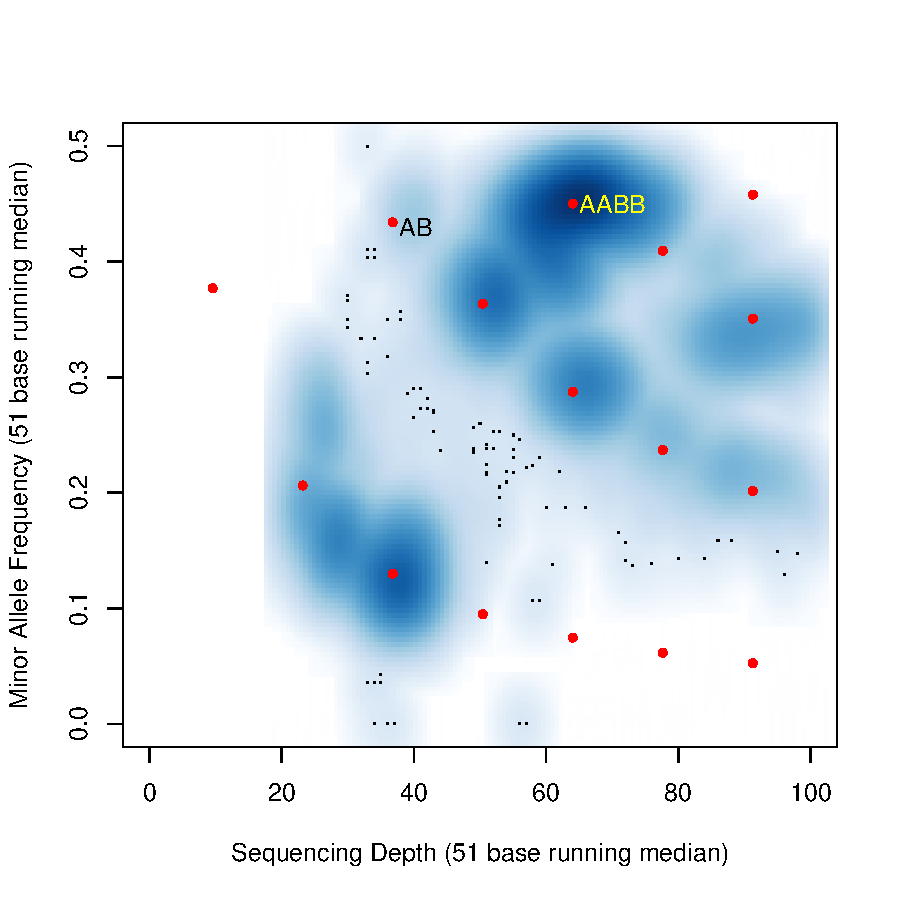
\includegraphics[width=\textwidth]{SS6003314.pdf}
\end{center}
\caption{A plot of minor allele fraction against sequencing depth reveals regions of consistent copy number.}
\label{Tumourexample}
\end{figure}

We load in Picard data for the entire library (duplicate rate: $5.2\%$), and for two sets of regions: i) The regions that are classified as AB (after removing masked regions - duplicate rate: $3.7\%$), and ii) The regions that are classified as AABB (after removing masked regions - duplicate rate: $3.8\%$). Note that this is a low duplication rate compared to those observed in libraries from normal tissue/blood. We attribute the change going from the entire library to the subsets as being due to the removal of masked regions; the AABB regions alone represent more than half of the sequencing library. We expect there to be a higher duplication rate in the AABB regions than in the AB region because of fragmentation duplicates. That it is such a small change suggests that the fragmentation duplicate rate will be small in this case.

\begin{Schunk}
\begin{Sinput}
> TumourPicard<-read.csv(file.path(EDpath,"Tumour","Picard.csv"),as.is=T)
> TumourPicard
\end{Sinput}
\begin{Soutput}
         LIBRARY UNPAIRED_READS_EXAMINED READ_PAIRS_EXAMINED UNMAPPED_READS
1      SS6003314                10432535           994242462       61864339
2   SS6003314-AB                    1576              417850           1576
3 SS6003314-AABB                 2438478           588331041        2438895
  UNPAIRED_READ_DUPLICATES READ_PAIR_DUPLICATES READ_PAIR_OPTICAL_DUPLICATES
1                  7153353             51808523                       455107
2                      402                15495                          188
3                   872992             22418117                       270067
  PERCENT_DUPLICATION ESTIMATED_LIBRARY_SIZE
1            0.055415             9281651350
2            0.037493                5558009
3            0.038766             7609634846
\end{Soutput}
\begin{Sinput}
> # and the duplicate rates
> round((TumourPicard[,6]-TumourPicard[,7])/(TumourPicard[,3]-TumourPicard[,7]),3)
\end{Sinput}
\begin{Soutput}
[1] 0.052 0.037 0.038
\end{Soutput}
\end{Schunk}

\subsection{The SNPs}

Tumour samples require bespoke lists, so we restrict ourselves to sites that we know to be heterozygous. We can define two sets of heterozygous SNPs for the AB ($985$ SNPs), and AABB (a sample of $10,000$ SNPs)  regions. 

\begin{Schunk}
\begin{Sinput}
> snplistAABB<-read.delim(file.path(EDpath,"Tumour","usedupAABB.txt"),as.is=T,header=F)
> snplistAB<-read.delim(file.path(EDpath,"Tumour","usedupAB.txt"),as.is=T,header=F)
\end{Sinput}
\end{Schunk}


\subsection{Counting the duplicates}

As before, we are unable to distribute the raw data, which are archived in the European Genome Archive [\href{https://www.ebi.ac.uk/ega/datasets/EGAD00001000704}{EGA:EGAD00001000704}]. The following code will generate the summary table in the manner we have come to expect.

\begin{Schunk}
\begin{Sinput}
> HetSNPTableAABB<-processBAMfordups("SS6003314.bam",path,snplistAABB,poscol=2)
> HetSNPTableAB<-processBAMfordups("SS6003314.bam",path,snplistAB,poscol=2)
> write.table(HetSNPTableAABB,file="HetSNPTableTumourAABB.txt",sep="\t")
> write.table(HetSNPTableAB,file="HetSNPTableTumourAB.txt",sep="\t")
\end{Sinput}
\end{Schunk}

Assuming that the user hasn't obtained the raw data, we now load in the precompiled summary table. Note that although we have pre-specified sites that are heterozygous, the filters in processBAMfordups have reduced the numbers to 8396 and 759.

\begin{Schunk}
\begin{Sinput}
> #HetSNPTableAABB<-read.delim(file.path(EDpath,"Tumour","HetSNPTableTumourAABB.txt"),as.is=T,header=T)
> #HetSNPTableAB<-read.delim(file.path(EDpath,"Tumour","HetSNPTableTumourAB.txt"),as.is=T,header=T)
> HetSNPTableAABB<-read.delim(file.path(EDpath,"HetSNPTableTumourAABB.tsv"),as.is=T,header=T)
> HetSNPTableAB<-read.delim(file.path(EDpath,"HetSNPTableTumourAB.tsv"),as.is=T,header=T)
> HetSNPTableTumour<-rbind(HetSNPTableAABB,HetSNPTableAB)
> rownames(HetSNPTableTumour)<-c("AABB","AB")
> rm(HetSNPTableAB,HetSNPTableAABB)
\end{Sinput}
\end{Schunk}

\subsection{Estimating the fragmentation duplicate proportion}

Processing this in the same manner as previous allele pattern counts...

\begin{Schunk}
\begin{Sinput}
> tumourresults<-processduptable(HetSNPTableTumour,PL,CL)
\end{Sinput}
\end{Schunk}

...we see that the fragmentation duplicate rate is higher in the AABB region than the AB region.

\begin{Schunk}
\begin{Sinput}
> tumourresults
\end{Sinput}
\begin{Soutput}
     ObservedDupRate PropFragDups AdjustedDupRate FragDupRate
AABB        3.755750        0.047        3.579230  0.17652026
AB          3.683342        0.017        3.620726  0.06261682
\end{Soutput}
\end{Schunk}




The difference between the two estimates has close to halved. Given the noise inherrent in the estimate from the smaller AB region, the corrected estimates from the AABB and AB regions are remarkably consistent.

\subsection{Extending to regions that are not in allelic balance}

We have demonstrated the approach only in genomic regions of allelic balance, but in theory this could be extended to any region where both alleles are present in the library (which due to contamination from normal cells, will still allow for regions that exhibit loss of heterozygosity in the tumour). 

The added complication comes in the form of $\Pr(AP_k \mid \text{PART}_i)$ (see section \ref{subsec:Case2}). Consider the case where we have two duplicate reads from the partition into two different molecules. Without loss of generailty let the alleles at the SNP of interest be C and T. Currently we only consider two possible allele patterns \texttt{AA} representing the posibilities CC and TT and \texttt{AB} representing CT and TC. Since the probability of each allele is $\frac{1}{2}$ we say that the probability of the \texttt{AA} pattern is also $\frac{1}{2} = 0.5^2 + 0.5^2$. 

Now if the allelic proportions are in fact $0.25$ and $0.75$, then we have two options:

\begin{itemize}

\item We still consider only two allele patterns, but the probability of the AA pattern is now $0.25^2 + 0.75^2 = 0.625$

\item We can confidently associate probabilities with specific alleles (e.g through phasing we may be confident that it is the C allele present in $75\%$ of molecules) in which case we would now consider three allele patterns \texttt{CC}, \texttt{CT}, \texttt{TT} with probabilities $0.5625$, $0.375$ and $0.0625$ respectively.

\end{itemize}

The second option is more powerful than the first, but would require a not insubstantial effort to ensure that the probabilities are matched to SNPs correctly. In both cases, since fragmentation duplicates are more inclined to share the same allele than when we have allelic balance, the analysis will be less powerful than when we have allelic balance. In studies of human tumours we have thus far always been able to identify regions of the genome in allelic balance, but we acknowledge that there is the potential need to go down this route of studying regions of allelic imbalance, and that indeed it may be a prerequisite for application of these methods to other organisms.

Note that for any sizeable segment of genome in the same state, we can empirically estimate the allelic fraction with enough precision that our methods will be useful, and so this does not cause problems.

\clearpage{}


\section{Complexity estimates}
% !Rnw root = duplicatessweave.Rnw

If the library complexity is $X$, the number of read-pairs sequenced is $N$, and the  duplicate rate is denoted by $R_D$, then our estimate of $X$ is obtained by solving
\begin{equation}  \label{calcX}
R_D = \frac{X}{N}\exp\left(-\frac{N}{X}\right)+1-\frac{X}{N}
\end{equation}
\noindent using numerical methods. See Lunter (\url{http://www.newton.ac.uk/programmes/
CGR/seminars/2010071310454.html}) for a derivation.

\subsection{Picard}

Picard bases its estimate of complexity on a genome-wide estimate of duplicate rate that is adversely affected by fragmentation duplicates.

\begin{Schunk}
\begin{Sinput}
> CEPicard<-unmaskedP[,9]
> summary(CEPicard)
\end{Sinput}
\begin{Soutput}
     Min.   1st Qu.    Median      Mean   3rd Qu.      Max. 
3.590e+09 5.814e+09 7.568e+09 7.704e+09 8.988e+09 1.355e+10 
\end{Soutput}
\end{Schunk}

\subsection{Estimating complexity using a basic duplication rate estimate}

We recalculate the complexity using the observed duplicate rate from the SNPs we interrogated. This corrects for the excessive influence of fragmentation duplicates in regions of high copy number/poor mappability, but not the general influence of fragmentation duplicates.

To obtain a starting point for the search, we use the closed form estimate based on a Maclaurin expansion $X = N/(2R_D)$.

\begin{Schunk}
\begin{Sinput}
> CEME<-rep(22,0)
> for(i in 1:22){
+   R<-FDres[i,1]/100
+   CEME[i]<-(readPairsExamined[i,1]-OpticalPairDuplicates[i,1])/(2*R)
+ }
\end{Sinput}
\end{Schunk}
 
Now we obtain our complexity estimates.

\begin{Schunk}
\begin{Sinput}
> CEobserved<-rep(22,0)
> for(i in 1:22){
+   R<-FDres[i,1]/100
+   N<-readPairsExamined[i,1]-OpticalPairDuplicates[i,1]
+   startX<-CEME[i]
+   CEobserved[i]<-optimize(libCompNewParam,R=R,N=N,interval=c(0,2*startX),maximum=F)$minimum
+ }
> summary(CEobserved)
\end{Sinput}
\begin{Soutput}
     Min.   1st Qu.    Median      Mean   3rd Qu.      Max. 
4.392e+09 7.950e+09 1.068e+10 1.259e+10 1.370e+10 2.853e+10 
\end{Soutput}
\end{Schunk}


In general the values are higher reflecting the lower duplicate rate estimate.

\subsection{Estimating complexity using a corrected duplication rate estimate}

This is the best estimate we can produce.

\begin{Schunk}
\begin{Sinput}
> CEcorrected<-rep(22,0)
> for(i in 1:22){
+   R<-FDres[i,3]/100
+   N<-readPairsExamined[i,1]-OpticalPairDuplicates[i,1]
+   startX<-CEME[i]
+   CEcorrected[i]<-optimize(libCompNewParam,R=R,N=N,interval=c(0,2*startX),maximum=F)$minimum
+ }
> summary(CEcorrected)
\end{Sinput}
\begin{Soutput}
     Min.   1st Qu.    Median      Mean   3rd Qu.      Max. 
4.490e+09 8.521e+09 1.116e+10 1.420e+10 1.508e+10 3.567e+10 
\end{Soutput}
\end{Schunk}



In all cases the standard estimate from Picard is lower than our best estimate of the library complexity (with factors ranging from 1.21 to 2.87) 
  
\begin{Schunk}
\begin{Sinput}
> summary(CEcorrected/CEPicard)
\end{Sinput}
\begin{Soutput}
   Min. 1st Qu.  Median    Mean 3rd Qu.    Max. 
  1.182   1.403   1.502   1.697   1.743   2.631 
\end{Soutput}
\end{Schunk}
  
\clearpage{}


\section{Adding additional lanes of sequencing}
% !Rnw root = duplicatessweave.Rnw

We now consider the effects of adding additional lanes of sequencing on estimates of complexity. First loading the Picard estimates, we see that the estimate of complexity increases with each lane.

\begin{Schunk}
\begin{Sinput}
> PicardLane<-read.delim(file.path(EDpath,"Picard", "SS6003301_lanes.metrics.txt"),as.is=T)
> PicardLane[,9]
\end{Sinput}
\begin{Soutput}
[1] 4864861694 5876377366 6510297164 6933459855 7273503256
\end{Soutput}
\begin{Sinput}
> round(PicardLane[,9]/PicardLane[5,9],2)
\end{Sinput}
\begin{Soutput}
[1] 0.67 0.81 0.90 0.95 1.00
\end{Soutput}
\end{Schunk}

We now apply our methods. As before, we are unable to distribute the raw data, which are archived in the European Genome Archive [\href{https://www.ebi.ac.uk/ega/datasets/EGAD00001000704}{EGA:EGAD00001000704}]. Upon obtaining the data, the following code would produce the required table.

\begin{Schunk}
\begin{Sinput}
> lanelist<-list(c("HSQ1004_100:1"),
+ c("HSQ1004_100:1","HSQ1004_100:2"),
+ c("HSQ1004_100:1","HSQ1004_100:2","HSQ1004_100:3"),
+ c("HSQ1004_100:1","HSQ1004_100:2","HSQ1004_100:3","HSQ1004_100:4"),
+ c("HSQ1004_100:1","HSQ1004_100:2","HSQ1004_100:3","HSQ1004_100:4","HSQ1004_97:8:"))
> HetSNPTableByLane<-processBAMbylane("SS6003301.bam",path,snplist,lanelist)
> write.table(HetSNPTableByLane,file="HetSNPDupsByLane.txt",sep="\t")
\end{Sinput}
\end{Schunk}

We now load and process the prepared table

\begin{Schunk}
\begin{Sinput}
> HetSNPTableByLane<-read.delim(file.path(EDpath,"HetSNPDupsByLane.txt"),as.is=T,header=T)
> EstimatesByLane<-processduptable(HetSNPTableByLane,PL,CL)
\end{Sinput}
\end{Schunk}

We generate a first order complexity estimate from which to begin our search.

\begin{Schunk}
\begin{Sinput}
> LaneCEME<-rep(0,5)
> for(i in 1:5){
+   R<-EstimatesByLane[i,1]/100
+   LaneCEME[i]<-(PicardLane[i,3]-PicardLane[i,7])/(2*R)
+ }
\end{Sinput}
\end{Schunk}

Now we generate complexity estimates using the observed duplicate rate from our heterozygous SNPs. Note that a) as expected from the previous section, the estimates are substantially greater, and b) the estimates are still monotonic but with a suggestion that they might be converging more quickly.


\begin{Schunk}
\begin{Sinput}
> LaneCEobserved<-rep(0,5)
> for(i in 1:5){
+   R<-EstimatesByLane[i,1]/100
+   N<-(PicardLane[i,3]-PicardLane[i,7])
+   startX<-LaneCEME[i]
+   LaneCEobserved[i]<-optimize(libCompNewParam,R=R,N=N,interval=c(0,2*startX),maximum=F)$minimum
+ }
> LaneCEobserved
\end{Sinput}
\begin{Soutput}
[1]  7847379090  8965708035  9607168600  9946088681 10350952077
\end{Soutput}
\begin{Sinput}
> round(LaneCEobserved/LaneCEobserved[5],2)
\end{Sinput}
\begin{Soutput}
[1] 0.76 0.87 0.93 0.96 1.00
\end{Soutput}
\end{Schunk}

Now we generate complexity estimates using the corrected duplicate rate.

\begin{Schunk}
\begin{Sinput}
> LaneCEcorrected<-rep(0,5)
> for(i in 1:5){
+   R<-EstimatesByLane[i,3]/100
+   N<-(PicardLane[i,3]-PicardLane[i,7])
+   startX<-LaneCEME[i]
+   LaneCEcorrected[i]<-optimize(libCompNewParam,R=R,N=N,interval=c(0,2*startX),maximum=F)$minimum
+ }
> LaneCEcorrected
\end{Sinput}
\begin{Soutput}
[1]  7975943131  9474139520 10100599958 10392584962 10817912779
\end{Soutput}
\begin{Sinput}
> round(LaneCEcorrected/LaneCEcorrected[5],2)
\end{Sinput}
\begin{Soutput}
[1] 0.74 0.88 0.93 0.96 1.00
\end{Soutput}
\end{Schunk}



\begin{Schunk}
\begin{Sinput}
> par(mfrow=c(1,2))
> plot(c(1,3),c(3,35),type="n",ylab="Library complexity estimate (billions)",xlab="",axes=F)
> axis(2)
> box()
> for(i in seq(0,40,2)){
+   rect(-1,i-1,5,i,border="grey95",col="grey95")
+ }
> for(i in 1:22){
+   tcol<-"black"
+   if(WeaverSuppTable1[i,12]=="Blood"){tcol<-"red"}
+   lines(1:3,c(CEPicard[i],CEobserved[i],CEcorrected[i])/(10^9),type="b",pch=16,col=tcol)
+ }
> axis(1,at=1:3,labels=c("Picard",
+                        "SNP observed",
+                        "Corrected"),las=3)
> plot(PicardLane[,9]/(10^9),pch=16,ylim=c(0,11),ylab="",xlab="Number of lanes",las=1,main="Complexity")
> points(LaneCEobserved/(10^9),pch=16,col="red")
> points(LaneCEcorrected/(10^9),pch=16,col="blue")
> legend("bottom",fill=c("black","red","blue"),legend=c("Picard","SNP\nobserved","SNP corrected"))
\end{Sinput}
\end{Schunk}
\incfig[!h]{duplicatessweave-Bylane7}{0.7\textwidth}{Consistency of estimates from sets of 2 fragments and sets of more than 2 fragments.}


\clearpage{}


\section{Mitochondria}
% !Rnw root = duplicatessweave.Rnw

The mitochondrial DNA poses an interesting problem as while it may exhibit heteroplasmy, it lacks sites that are heterozygous with predictable allele fractions, but at the same time often has such high copy number that the coincedental fragmentation duplicates are a large problem.

\subsection{Simulation}

We begin by simulating mitochondrial reads to determine the extent of the problem. We investigate various copy numbers, and use our two extreme insert size distribtuions. We also simulate single end sequencing, by halving the length of the reads and allowing no variation in insert sizes.

\begin{Schunk}
\begin{Sinput}
> set.seed(246810)
> NarrowMTres<-simMTreads(numcopies=100,realISD=ISDnarrow)
> NarrowMTres<-rbind(NarrowMTres,simMTreads(numcopies=200,realISD=ISDnarrow))
> NarrowMTres<-rbind(NarrowMTres,simMTreads(numcopies=300,realISD=ISDnarrow))
> NarrowMTres<-rbind(NarrowMTres,simMTreads(numcopies=400,realISD=ISDnarrow))
> NarrowMTres<-rbind(NarrowMTres,simMTreads(numcopies=500,realISD=ISDnarrow))
> NarrowMTres<-rbind(NarrowMTres,simMTreads(numcopies=600,realISD=ISDnarrow))
> NarrowMTres<-rbind(NarrowMTres,simMTreads(numcopies=700,realISD=ISDnarrow))
> NarrowMTres<-rbind(NarrowMTres,simMTreads(numcopies=800,realISD=ISDnarrow))
> NarrowMTres<-rbind(NarrowMTres,simMTreads(numcopies=900,realISD=ISDnarrow))
> NarrowMTres<-rbind(NarrowMTres,simMTreads(numcopies=1000,realISD=ISDnarrow))
> WideMTres<-simMTreads(numcopies=100,realISD=ISDwide)
> WideMTres<-rbind(WideMTres,simMTreads(numcopies=200,realISD=ISDwide))
> WideMTres<-rbind(WideMTres,simMTreads(numcopies=300,realISD=ISDwide))
> WideMTres<-rbind(WideMTres,simMTreads(numcopies=400,realISD=ISDwide))
> WideMTres<-rbind(WideMTres,simMTreads(numcopies=500,realISD=ISDwide))
> WideMTres<-rbind(WideMTres,simMTreads(numcopies=600,realISD=ISDwide))
> WideMTres<-rbind(WideMTres,simMTreads(numcopies=700,realISD=ISDwide))
> WideMTres<-rbind(WideMTres,simMTreads(numcopies=800,realISD=ISDwide))
> WideMTres<-rbind(WideMTres,simMTreads(numcopies=900,realISD=ISDwide))
> WideMTres<-rbind(WideMTres,simMTreads(numcopies=1000,realISD=ISDwide))
> SEMTres<-simMTreads(numcopies=100,ISmean=100,ISsd=0,readlength=50)
> SEMTres<-rbind(SEMTres,simMTreads(numcopies=200,ISmean=100,ISsd=0,readlength=50))
> SEMTres<-rbind(SEMTres,simMTreads(numcopies=300,ISmean=100,ISsd=0,readlength=50))
> SEMTres<-rbind(SEMTres,simMTreads(numcopies=400,ISmean=100,ISsd=0,readlength=50))
> SEMTres<-rbind(SEMTres,simMTreads(numcopies=500,ISmean=100,ISsd=0,readlength=50))
> SEMTres<-rbind(SEMTres,simMTreads(numcopies=600,ISmean=100,ISsd=0,readlength=50))
> SEMTres<-rbind(SEMTres,simMTreads(numcopies=700,ISmean=100,ISsd=0,readlength=50))
> SEMTres<-rbind(SEMTres,simMTreads(numcopies=800,ISmean=100,ISsd=0,readlength=50))
> SEMTres<-rbind(SEMTres,simMTreads(numcopies=900,ISmean=100,ISsd=0,readlength=50))
> SEMTres<-rbind(SEMTres,simMTreads(numcopies=1000,ISmean=100,ISsd=0,readlength=50))
\end{Sinput}
\end{Schunk}


In Figure~\ref{duplicatessweave-MTDNA} we see that with a tight insert size distribution more than half of the reads can be marked as duplicates despite not being PCR duplicates. Moreover, comparing copy numbers between samples is hampered by the saturation effect that compresses the dynamic range, and particularly by differences between the insert size distributions, if one adopts the common practise of removing all `duplicates'.


\subsection{Picard}

We revisit the Picard output from the mitochondrial mask discussed in the ``Sample Information'' section. In doing so we will create an object entitled \texttt{PicardMito} as described below.

\begin{Schunk}
\begin{Sinput}
> lf<-read.delim(file.path(EDpath,"Picard",metfiles[3]),as.is=T)
> lf<-lf[-(15:19),]
\end{Sinput}
\end{Schunk}

The Picard duplicate rate is inflated by up to 3\% by the inclusion of`unpaired' reads in its calculation (these are virtually all marked as duplicates in the high-copy context of the mtDNA). However it indicates that on average a third of reads (and up to two-thirds of reads) are marked as duplicates, and since we have a good estimate of the true PCR duplicate rate we can see that the apparent rate in the mitochondria inflates this by a factor of up to $36\times$

\begin{Schunk}
\begin{Sinput}
> summary(lf[,8])
\end{Sinput}
\begin{Soutput}
   Min. 1st Qu.  Median    Mean 3rd Qu.    Max. 
 0.1446  0.1966  0.2608  0.3200  0.4042  0.6591 
\end{Soutput}
\begin{Sinput}
> summary(100*lf[,8]/FDres[,3])
\end{Sinput}
\begin{Soutput}
   Min. 1st Qu.  Median    Mean 3rd Qu.    Max. 
  3.378   4.444   6.766   8.187   9.506  35.920 
\end{Soutput}
\end{Schunk}

We now tabulate the depth of sequencing with and without removing duplicates, and also with our correction for the PCR duplicate rate

\begin{Schunk}
\begin{Sinput}
> MitoDepths<-cbind(lf[,3]*200+lf[,2]*100,lf[,3]*200+lf[,2]*100-lf[,6]*200-lf[,5]*100,(lf[,3]*200+lf[,2]*100)*(100-FDres[,3])/100)/16569
> MitoCNs<-MitoDepths/(ResDepth*(100-FDres[,3])/200)
> 
\end{Sinput}
\end{Schunk}

Now we produce Figure 3 from the paper (Figure \ref{duplicatessweave-AddFig3} in this document), combining complexity and mitochondrial copy number results.

\begin{Schunk}
\begin{Sinput}
> par(mfrow=c(1,2))
> plot(as.numeric(NarrowMTres[,8]),as.numeric(NarrowMTres[,9]),xlim=c(0,1000),ylim=c(0,1000),pch=16,type="b",xlab="True copy number",ylab="Inferred copy number",main="Simulations")
> points(as.numeric(WideMTres[,8]),as.numeric(WideMTres[,9]),col="red",pch=16,type="b")
> points(as.numeric(SEMTres[,8]),as.numeric(SEMTres[,9]),col="blue",pch=16,type="b")
> abline(0,1,lwd=2)
> legend("topleft",fill=c("red","black","blue"),legend=c("Wide ISD","Narrow ISD","Single end"))
> lines(c(-100,900),c(383,383),lty=3,col="black",lwd=2)
> lines(c(-100,500),c(397,397),lty=3,col="red",lwd=2)
> lines(c(900,900),c(-100,383),lty=3,col="black",lwd=2)
> lines(c(500,500),c(-100,397),lty=3,col="red",lwd=2)
> plot(c(1,3),c(60,800),type="n",ylab="MtDNA copy number",xlab="",axes=F,main="Our 22 Example Cases")
> axis(2)
> box()
> for(i in seq(0,800,200)){
+   rect(-1,i-100,5,i,border="grey95",col="grey95")
+ }
> for(i in 1:22){
+   tcol<-"black"
+   if(WeaverSuppTable1[i,12]=="Blood"){tcol<-"red"}
+   lines(1:3,(as.numeric(MitoCNs[i,c(1,3,2)])),type="b",pch=16,col=tcol)
+ }
> axis(1,at=1:3,labels=c("No\nduplicates\nremoved","Corrected\nestimate","All\nduplicates\nremoved"),las=3)
\end{Sinput}
\end{Schunk}
\incfig[htbp!]{duplicatessweave-MTDNA}{\textwidth}{mtDNA copy number results}{Text text text}


\clearpage{}

\section{Session Info}

For updates to this package/document, please visit www.compbio.group.cam.ac.uk.

\begin{Schunk}
\begin{Sinput}
> toLatex(sessionInfo())
\end{Sinput}
\begin{itemize}\raggedright
  \item R version 3.2.3 (2015-12-10), \verb|x86_64-apple-darwin13.4.0|
  \item Locale: \verb|en_GB.UTF-8/en_GB.UTF-8/en_GB.UTF-8/C/en_GB.UTF-8/en_GB.UTF-8|
  \item Base packages: base, datasets, graphics, grDevices, methods, parallel,
    stats, stats4, utils
  \item Other packages: BiocGenerics~0.16.1, Biostrings~2.38.4, BSgenome~1.38.0,
    BSgenome.Hsapiens.UCSC.hg19~1.4.0, FragmentationDuplicates~0.9,
    GenomeInfoDb~1.6.3, GenomicRanges~1.22.4, IRanges~2.4.8, Rsamtools~1.22.0,
    rtracklayer~1.30.3, S4Vectors~0.8.11, xtable~1.8-2, XVector~0.10.0
  \item Loaded via a namespace (and not attached): Biobase~2.30.0,
    BiocParallel~1.4.3, BiocStyle~1.8.0, bitops~1.0-6, futile.logger~1.4.1,
    futile.options~1.0.0, GenomicAlignments~1.6.3, lambda.r~1.1.7,
    RCurl~1.95-4.8, SummarizedExperiment~1.0.2, tools~3.2.3, XML~3.98-1.4,
    zlibbioc~1.16.0
\end{itemize}\end{Schunk}

\end{document}
